%% Requires compilation with XeLaTeX or LuaLaTeX
\documentclass[compress,10pt,xcolor={table,dvipsnames},t]{beamer} %aspectratio=169
\usetheme{diapo}
\usepackage{amsmath}
\DeclareMathOperator*{\argmax}{arg\,max}
\DeclareMathOperator*{\argmin}{argmin}
\usepackage{xparse} %for \NewDocumentEnvironment
\usepackage{amssymb}
\usepackage{xcolor}
\usepackage[bottom]{footmisc}
\usepackage{multirow}
\usepackage{setspace}
\usepackage{caption}
\usepackage{array,multirow,makecell}
\usepackage{pifont}
\usepackage{tikz}
\usepackage{paralist}
\usepackage{appendixnumberbeamer}
%\usepackage[style=authoryear,sorting=nyt,doi=false,url=false,maxbibnames=99,date=year]{biblatex}
\usepackage[square]{natbib}
\bibliographystyle{plainnat}
\usepackage{etoolbox}
% box colorée dans équation
\usepackage[most]{tcolorbox}
\usepackage{tikz}
\usepackage{soul}
% pour l'indicatrice
\usepackage{dsfont}
\usepackage{cancel}
\usepackage{booktabs}
\usepackage{bm}
% pour indentation des itemize
% \usepackage{enumitem}

\setcellgapes{1pt}
\setlength{\parindent}{0pt}
\makegapedcells
\newcolumntype{R}[1]{>{\raggedleft\arraybackslash }b{#1}}
\newcolumntype{L}[1]{>{\raggedright\arraybackslash }b{#1}}
\newcolumntype{C}[1]{>{\centering\arraybackslash }b{#1}}
\renewcommand*{\bibfont}{\footnotesize}
\useoutertheme[subsection=false]{miniframes}
\makeatletter
%\patchcmd{\slideentry}{\advance\beamer@xpos by1\relax}{}{}{}
\def\beamer@subsectionentry#1#2#3#4#5{\advance\beamer@xpos by1\relax}%
\makeatother
\setbeamercolor*{mini frame}{fg=bulles,bg=bulles}
\hypersetup{
	colorlinks=true,
	urlcolor=blue,
	citecolor=other,
	linkcolor=title,
}

\title[PhiFEM]{Enriching continuous Lagrange finite element approximation spaces using neural networks}
\subtitle{ICOSAHOM 2025}

\author{%
	Michel Duprez\inst{1}, 
	Emmanuel Franck\inst{2},
	\textbf{Frédérique Lecourtier}\inst{1} and
    Vanessa Lleras\inst{3}
}


\institute{%
	\inst{1} Project-Team MIMESIS, Inria, Strasbourg, France \\
    \inst{2} Project-Team MACARON, Inria, Strasbourg, France \\
    \inst{3} IMAG, University of Montpellier, Montpellier, France
}

\date{July 15, 2025}

\allowbreak

% u_chapeau (chapeau en couleur)
\usepackage{accents}
\newcommand{\uchapeau}[1]{\accentset{\textcolor{red}{\wedge}}{#1}}
\newcommand{\refappendix}[1]{\tikz[baseline=(char.base)]{\node[framednumber] (char) {\hyperlink{#1}{\small \textcolor{white}{Appendix \ref*{#1}}}};}}
% \newcommand{\refsubappendix}[1]{\tikz[baseline=(char.base)]{\node[framednumber] (char) {\hyperlink{#1.maj}{\small \textcolor{white}{Appendix \ref*{#1}}}};}}

\tikzset{
	framednumber/.style={
		draw=appendix,% Couleur de la bordure
		fill=appendix, % Couleur de fond
		rounded corners, % Coins arrondis
		inner sep=2pt,  % Espace intérieur
	}
}

%% numérotation et label des appendix
\newcounter{appendixframenumber}
\setcounter{appendixframenumber}{0}
\newcounter{subappendixframenumber}
\setcounter{subappendixframenumber}{1}

\makeatletter
\newcommand{\labelappendixframe}[1]{%
	\protected@write\@auxout{}{%
		\string\newlabel{#1}{{\theappendixframenumber}{\thepage}}%
	}%
	\hypertarget{#1}{}
}	
\makeatother

% Ce compteur temporaire stockera "x.y" (1.1, 1.2, etc.) pour les sous-appendices
\makeatletter
\newcommand{\labelsubappendixframe}[1]{%
	\edef\@currentlabel{\theappendixframenumber.\thesubappendixframenumber}%
	\label{#1}%
}
\makeatother

\newcommand{\appendixsection}[1]{%
	\addtocounter{appendixframenumber}{1}%
	\section{\appendixname~\theappendixframenumber~: #1}%\labelappendixframe{frame:#2}%
	\setcounter{subappendixframenumber}{1}% Réinitialiser le compteur des sous-appendices
}

\NewDocumentEnvironment{subappendixframe}{mo+b} 
{%
	% Optionnal : noframenumbering
	\IfNoValueTF{#2}
	{\begin{frame}{A\theappendixframenumber.\thesubappendixframenumber~– #1}}
	{\begin{frame}[#2]{A\theappendixframenumber.\thesubappendixframenumber~– #1}}
		#3
	\end{frame}
}{}

\NewDocumentEnvironment{appendixframe}{mo+b} 
{%
	% Optionnal : noframenumbering
	\IfNoValueTF{#2}
	{\begin{frame}{A\theappendixframenumber~– #1}}
	{\begin{frame}[#2]{A\theappendixframenumber~– #1}}
		#3
	\end{frame}
}{}

% barre en couleur terme dans équation
\newcommand\Ccancel[2][black]{\renewcommand\CancelColor{\color{#1}}\cancel{#2}}

% chifrre romain dans le texte
\makeatletter
\newcommand*{\rom}[1]{\expandafter\@slowromancap\romannumeral #1@}
\makeatother

% warning
\newcommand{\warning}{{\fontencoding{U}\fontfamily{futs}\selectfont\char 49\relax}}

\newcommand{\insertsectionheadSubtitle}{}

\newtcbtheorem{mytheo}{Theorem}{colback=other, % Couleur de fond de la boîte
	colframe=other, % Couleur du cadre de la boîte
	arc=2mm, % Rayon de l'arrondi des coins
	boxrule=0.5pt, % Épaisseur du cadre de la boîte
	breakable, enhanced jigsaw,
	width=\linewidth,
	opacityback=0.1
	}{th}

\newcommand*{\footcite}[1]{\footnote[frame,1]{\citep{#1}}}

% star command
\newcommand{\filledstar}{\textcolor{Goldenrod}{\ding{72}}\hspace{-8pt}\ding{73}\,}

\definecolor{flechecolor}{rgb}{0, 0, 1}
\newcommand{\flechecourbe}[5]{%
  % #1 = abscisse de départ (x)
  % #2 = ordonnée de départ (y)
  % #3 = taille en abscisse de la flèche (x)
  % #4 = taille en ordonnée de la flèche (y)
  % #5 = texte à mettre au centre
  \draw[thick,->,flechecolor]
    (#1,#2) .. controls (#1+0.4*#3,#2+#4) and (#1+0.6*#3,#2+#4) .. (#1+#3,#2)
    node[midway, sloped, fill=white, inner sep=1pt] {\tiny #5};
}

% algorithm
\usepackage[ruled,vlined]{algorithm2e}
\usepackage{multirow}

% define color : darkred : red!85!black
\definecolor{darkred}{rgb}{0.9, 0, 0}


\usepackage{amssymb}
\usepackage{mathtools}
\usepackage{pgfplots}
\usepackage{pgfplotstable}
% \usepackage{filecontents}
\usepackage{datatool}
\usepackage{fp}
\usetikzlibrary{backgrounds}

\pgfplotsset{
    compat=newest,
}
\pgfplotsset{
    smaller labels/.style={
        label style={font=\footnotesize},
        tick label style={font=\footnotesize}
    }
}
\tikzset{font=\small}
\usetikzlibrary{
    fpu,
    fixedpointarithmetic,
    babel,
    external,
    arrows.meta,
    plotmarks,
    positioning,
    angles,
    quotes,
    intersections,
    calc,
    spy,
    decorations.pathreplacing,
    matrix,
    fit,
}
\usepgfplotslibrary{fillbetween}

% Define colors
\definecolor{femcolor}{RGB}{51, 138, 55} %Green (27,158,119)
\definecolor{addcolor}{RGB}{217,95,2} %Orange
\definecolor{addsobcolor}{RGB}{199,39,34} %Red (sob or other)
\definecolor{multcolor3}{RGB}{117,112,179} %Purple 
\definecolor{multcolor100}{RGB}{0,0,0} %Black (+ empty marker)
\definecolor{multcolor0weak}{RGB}{49, 73, 181} %Blue
\definecolor{multcolor0strong}{RGB}{49, 181, 161} %Cyan

% Define line styles according to the method 
% FEM : solid
% Add : dashed
% Mult : dotted

% Define marker styles according to the degree
% P1 : square
% P2 : circle
% P3 : triangle

%________________ error lines (by Ricardo Costa) ________________

% argument 1: slopes (e.g. {4,6})
% argument 2: x position of the bottom left corner
% argument 3: y position of the bottom left corner
% argument 4: x length

\makeatletter

\newcommand{\printslopeinv}[4]{
    \tikzset{fixed point arithmetic}
    % get arguments
    \def\nero@printslope@orderlist{#1}
    \edef\nero@printslope@xpos{#2}
    \edef\nero@printslope@ypos{#3}
    \edef\nero@printslope@width{#4}
    % get points position
    \pgfmathparse{\nero@printslope@xpos+\nero@printslope@width}
    \edef\nero@printslope@px{\pgfmathresult}
    \edef\nero@printslope@py{\nero@printslope@ypos}
    \edef\nero@printslope@qx{\pgfmathresult}
    \edef\nero@printslope@ry{\nero@printslope@ypos}
    \foreach \nero@printslope@order in {#1}{
        \pgfmathparse{
        ((\nero@printslope@px/\nero@printslope@xpos)^(\nero@printslope@order))*\nero@printslope@ypos}
        \edef\nero@printslope@qy{\pgfmathresult}
            \edef\nero@aux1{\noexpand\draw[line width=0.6pt]
            (axis cs:\nero@printslope@xpos,\nero@printslope@ypos)
            -- (axis cs:\nero@printslope@qx,\nero@printslope@qy)
            -- (axis cs:\nero@printslope@px,\nero@printslope@py);}
        \nero@aux1
        % slope label
        \pgfmathparse{10^((ln(\nero@printslope@ry)+ln(\nero@printslope@qy))/(ln(10)*2))}
        \edef\nero@printslope@labelpos{\pgfmathresult}
        \edef\nero@aux2{\noexpand\node[anchor=west] at
            (axis cs:\nero@printslope@qx,\nero@printslope@labelpos)
            {\noexpand\tiny \nero@printslope@order};}
        \nero@aux2
        \global\edef\nero@printslope@ry{\nero@printslope@qy}
    }
    % base line
    \draw[line width=0.6pt] (axis cs:\nero@printslope@xpos,\nero@printslope@ypos)
        |- (axis cs:\nero@printslope@px,\nero@printslope@py);
    % label of base line
    \pgfmathparse{10^((ln(\nero@printslope@px)+ln(\nero@printslope@xpos))/(ln(10)*2))}
    \edef\nero@printslope@labelpos{\pgfmathresult}
    \node[anchor=north] at (axis cs:\nero@printslope@labelpos,\nero@printslope@ypos) {\tiny 1};
}

\makeatother

\newlength{\plotwidth}
\setlength{\plotwidth}{0.54\textwidth}
\newlength{\plotheight}
\setlength{\plotheight}{0.4\textwidth}

\gdef\iterator{0}

\newenvironment{cvgh}[4]{
    \begin{tikzpicture}
        \edef\filename{#1}
        \edef\legendcolumns{#2}
        \edef\slopes{#3}
        \edef\ypos{#4}

        % Read the CSV file into a table
        \pgfplotstableread[col sep=comma]{\filename}\datatable

        % Obtenir le second élément
        \pgfmathtruncatemacro{\secondrow}{1} % Index de la dernière ligne
        \pgfplotstablegetelem{\secondrow}{h}\of\datatable
        \pgfmathsetmacro{\second}{\pgfplotsretval} % Dernière valeur de h_rounded

        % Obtenir le premier élément
        \pgfmathtruncatemacro{\firstrow}{0} % Index de l'avant-dernière ligne
        \pgfplotstablegetelem{\firstrow}{h}\of\datatable
        \pgfmathsetmacro{\first}{\pgfplotsretval} % Avant-dernière valeur de h_rounded

        % Calculer la différence entre les deux
        \pgfmathsetmacro{\diff}{\first - \second}

        %update iterator
        \pgfmathtruncatemacro{\iterator}{\iterator+1}

        \begin{loglogaxis}[
            smaller labels,
            name = left_plot,
            % axis lines
            axis lines = left,
            enlarge x limits={abs=10pt},
            enlarge y limits={abs=10pt},
            % axis x line shift = -5pt,
            axis y line shift = -5pt,
            % labels
			xmode=log,
            xlabel = {$h$},
            ylabel = {\rotatebox{270}{$L^2$}},
            xlabel style={at={(ticklabel* cs:1.01)},anchor=west},
            ylabel style={at={(ticklabel* cs:1.01)},anchor=west},
            % ticks and labels
            xtick=data,
            xticklabels from table={\datatable}{h},
            width=\plotwidth, height=\plotheight,
            mark options={solid, scale=1},
            grid = major,
            legend columns=\legendcolumns,
            legend to name=leg:legendFEMCORR_\iterator,
            legend image post style={mark options={solid, scale=1},xscale=0.8},
        ]
        \expandafter\printslopeinv\expandafter{\slopes}{\second}{\ypos}{\diff}
    }
    {
        \end{loglogaxis}
        \node[yshift=-20pt] at (left_plot.outer south) {\pgfplotslegendfromname{leg:legendFEMCORR_\iterator}};

    \end{tikzpicture}
}

\newenvironment{cvghline}[4]{
    \begin{tikzpicture}
        \edef\filename{#1}
        \edef\legendcolumns{#2}
        \edef\slopes{#3}
        \edef\ypos{#4}

        % Read the CSV file into a table
        \pgfplotstableread[col sep=comma]{\filename}\datatable

        % Obtenir le second élément
        \pgfmathtruncatemacro{\secondrow}{1} % Index de la dernière ligne
        \pgfplotstablegetelem{\secondrow}{h}\of\datatable
        \pgfmathsetmacro{\second}{\pgfplotsretval} % Dernière valeur de h_rounded

        % Obtenir le premier élément
        \pgfmathtruncatemacro{\firstrow}{0} % Index de l'avant-dernière ligne
        \pgfplotstablegetelem{\firstrow}{h}\of\datatable
        \pgfmathsetmacro{\first}{\pgfplotsretval} % Avant-dernière valeur de h_rounded

        % Calculer la différence entre les deux
        \pgfmathsetmacro{\diff}{\first - \second}

        %update iterator
        \pgfmathtruncatemacro{\iterator}{\iterator+1}

        \begin{loglogaxis}[
            smaller labels,
            name = left_plot,
            % axis lines
            axis lines = left,
            enlarge x limits={abs=10pt},
            enlarge y limits={abs=10pt},
            % axis x line shift = -5pt,
            axis y line shift = -5pt,
            % labels
			xmode=log,
            xlabel = {$h$},
            ylabel = {\rotatebox{270}{$L^2$}},
            xlabel style={at={(ticklabel* cs:1.01)},anchor=west},
            ylabel style={at={(ticklabel* cs:1.01)},anchor=west},
            % ticks and labels
            xtick=data,
            xticklabels from table={\datatable}{h},
            width=\plotwidth, height=\plotheight,
            mark options={solid, scale=1},
            grid = major,
            legend columns=\legendcolumns,
            legend to name=leg:legendFEMCORR_\iterator,
            legend image post style={mark options={solid, scale=1},xscale=0.8},
        ]
        \expandafter\printslopeinv\expandafter{\slopes}{\second}{\ypos}{\diff}
    }
    {
        \end{loglogaxis}
        \node[yshift=-20pt] at (left_plot.outer south) {\pgfplotslegendfromname{leg:legendFEMCORR_\iterator}};
        
        \draw[black, line width=0.4mm] (0.1,1.9) -- (4.7,1.9) node[anchor=west, xshift=2pt] {$e$};

    \end{tikzpicture}
}

\newcommand{\cvgFEMCorrAlldeg}[3]{
    \edef\fem{#1}
    \edef\add{#2}

    \begin{cvgh}{\fem}{3}{2,3,4}{#3}
        % Complete the legend
        \addlegendentry{\,FEM $\mathbb{P}_1$\;}
        \addlegendentry{\,FEM $\mathbb{P}_2$\;}
        \addlegendentry{\,FEM $\mathbb{P}_3$\;}
        \addlegendentry{\,Add $\mathbb{P}_1$\;}
        \addlegendentry{\,Add $\mathbb{P}_2$\;}
        \addlegendentry{\,Add $\mathbb{P}_3$\;}

        % Plot FEM
        \addplot [style={solid}, mark=square*, mark size=2, color=femcolor, line width=0.8pt ]
        table [x=h, y=P1, col sep=comma]
            {\fem};
        
        \addplot [style={solid}, mark=*, mark size=2, color=femcolor, line width=0.8pt ]
        table [x=h, y=P2, col sep=comma]
            {\fem};
        
        \addplot [style={solid}, mark=triangle*, mark size=2, color=femcolor, line width=0.8pt ]
        table [x=h, y=P3, col sep=comma]
            {\fem};

        % Plot Add
        \addplot [style={dashed}, mark=square*, mark size=2, color=addcolor, line width=0.8pt ]
        table [x=h, y=P1, col sep=comma]
            {\add};

        \addplot [style={dashed}, mark=*, mark size=2, color=addcolor, line width=0.8pt ]
        table [x=h, y=P2, col sep=comma]
            {\add};

        \addplot [style={dashed}, mark=triangle*, mark size=2, color=addcolor, line width=0.8pt ]
        table [x=h, y=P3, col sep=comma]
            {\add};

    \end{cvgh}
}

\newcommand{\cvgFEMCorrAlldegLine}[3]{
    \edef\fem{#1}
    \edef\add{#2}

    \begin{cvghline}{\fem}{3}{2,3,4}{#3}
        % Complete the legend
        \addlegendentry{\,FEM $\mathbb{P}_1$\;}
        \addlegendentry{\,FEM $\mathbb{P}_2$\;}
        \addlegendentry{\,FEM $\mathbb{P}_3$\;}
        \addlegendentry{\,Add $\mathbb{P}_1$\;}
        \addlegendentry{\,Add $\mathbb{P}_2$\;}
        \addlegendentry{\,Add $\mathbb{P}_3$\;}

        % Plot FEM
        \addplot [style={solid}, mark=square*, mark size=2, color=femcolor, line width=0.8pt ]
        table [x=h, y=P1, col sep=comma]
            {\fem};
        
        \addplot [style={solid}, mark=*, mark size=2, color=femcolor, line width=0.8pt ]
        table [x=h, y=P2, col sep=comma]
            {\fem};
        
        \addplot [style={solid}, mark=triangle*, mark size=2, color=femcolor, line width=0.8pt ]
        table [x=h, y=P3, col sep=comma]
            {\fem};

        % Plot Add
        \addplot [style={dashed}, mark=square*, mark size=2, color=addcolor, line width=0.8pt ]
        table [x=h, y=P1, col sep=comma]
            {\add};

        \addplot [style={dashed}, mark=*, mark size=2, color=addcolor, line width=0.8pt ]
        table [x=h, y=P2, col sep=comma]
            {\add};

        \addplot [style={dashed}, mark=triangle*, mark size=2, color=addcolor, line width=0.8pt ]
        table [x=h, y=P3, col sep=comma]
            {\add};

    \end{cvghline}
}

\newcommand{\cvgFEMCorrMultOnedeg}[6]{
    \edef\fem{#1}
    \edef\femsec{#2}
    \edef\add{#3}
    \edef\mult{#4}
    \edef\multHundred{#5}

    \begin{cvgh}{\fem}{3}{2,3}{#6}
        % Complete the legend
        \addlegendentry{\,FEM $\mathbb{P}_1$\;}
        \addlegendentry{\,Mult $\mathbb{P}_1$ (M=3)\;}
        \addlegendentry{\,Add $\mathbb{P}_1$\;}
        \addlegendentry{\,FEM $\mathbb{P}_2$\;}
        \addlegendentry{\,Mult $\mathbb{P}_1$ (M=100)\;}

        % Plot the data
        \addplot [style={solid}, mark=square*, mark size=2, color=femcolor, line width=0.8pt ]
        table [x=h, y=err, col sep=comma]
            {\fem};

        \addplot [style={dotted}, mark=square*, mark size=2, color=multcolor3, line width=1.0pt ]
        table [x=h, y=err, col sep=comma]
            {\mult};

        \addplot [style={dashed}, mark=square*, mark size=2, color=addcolor, line width=0.8pt ]
        table [x=h, y=err, col sep=comma]
            {\add};

        \addplot [style={solid}, mark=*, mark size=2, color=femcolor, line width=0.8pt ]
        table [x=h, y=err, col sep=comma]
            {\femsec};

        \addplot [style={dotted}, mark=square, mark size=2, color=multcolor100, line width=1.0pt ]
        table [x=h, y=err, col sep=comma]
            {\multHundred};
    \end{cvgh}
}
\usepackage{booktabs}
\usepackage{xcolor}

% gains pour tous les q
\newcommand{\gainstableallq}[1]{
    \pgfplotstabletypeset[
        col sep=comma,
        every head row/.style={
        before row={\toprule[1.pt]
        & \multicolumn{3}{c}{\textbf{Gains in $L^2$ rel error}} \\
		& \multicolumn{3}{c}{\textbf{of our method w.r.t. FEM}} \\
		\cmidrule(lr){2-4}
        },
        after row=\cmidrule(lr){1-1} \cmidrule(lr){2-4}},
        every last row/.style={after row=\bottomrule[1.pt]},
        every nth row={1}{before row=\cmidrule(lr){1-1} \cmidrule(lr){2-4}},
		columns/q/.style={column name=\textbf{k}},
        columns/min_FEM/.style={column name=\textbf{min},fixed},
        columns/max_FEM/.style={column name=\textbf{max},fixed},
        columns/mean_FEM/.style={column name=\textbf{mean},fixed,
            postproc cell content/.append style={
                /pgfplots/table/@cell content/.add={\color{red}}{},
            }
        },
        columns={q,min_FEM,max_FEM,mean_FEM},
        precision=2
    ]{#1}
}


\usepackage{booktabs}

% costs pour tous les q : N et DoFs
\newcommand{\coststableallq}[1]{
    \pgfplotstabletypeset[
        col sep=comma,
        every head row/.style={
        before row={\toprule[1.pt]
        & & \multicolumn{2}{c}{\textbf{$N_\text{dofs}$}} \\
		\cmidrule(lr){3-4}
        },
        after row=\cmidrule(lr){1-1} \cmidrule(lr){2-2} \cmidrule(lr){3-4}},
        every last row/.style={after row=\bottomrule[1.pt]},
        every nth row={2}{before row=\cmidrule(lr){1-1} \cmidrule(lr){2-2} \cmidrule(lr){3-4}},
		columns/q/.style={column name=\textbf{k}},
        columns/e/.style={column name=\textbf{e},sci},
		columns/FEM_dofs/.style={column name=\textbf{FEM},fixed},
        columns/Add_dofs/.style={column name=\textbf{Add},fixed},
        columns={q,e,FEM_dofs,Add_dofs},
        precision=2
    ]{#1}
}

\begin{document}
	% \nocite{*}
	
	\renewcommand{\inserttotalframenumber}{\pageref{lastslide}}
	
	{\setbeamertemplate{footline}{} 
		\BackgroundTitle
		\begin{frame}[plain]
			\maketitle
		\end{frame}
	}
	\addtocounter{framenumber}{-1} 	
	
	\AtBeginSection[]{
		{\setbeamertemplate{footline}{}
			\begin{frame}
				\vfill
				\centering
				\begin{beamercolorbox}[sep=5pt,shadow=true,rounded=true]{subtitle}
					\usebeamerfont{title}\insertsectionhead\par%
					\vspace{0.5cm} % Ajustez l'espacement selon vos besoins
					% \usebeamerfont{classic}\usebeamercolor[fg]{classic}\insertsectionheadSubtitle
				\end{beamercolorbox}
				%\tableofcontents[sectionstyle=hide,subsectionstyle=show]
				
				%subsectionstyle=⟨style for current subsection⟩/⟨style for other subsections in current section⟩/⟨style for subsections in other sections⟩
				\tableofcontents[sectionstyle=hide,subsectionstyle=show/show/hide]
				\vfill
				\begin{beamercolorbox}[sep=5pt,shadow=true,rounded=true]{subtitle}
					\usebeamerfont{classic}\usebeamercolor[fg]{classic}\insertsectionheadSubtitle
				\end{beamercolorbox}
			\end{frame}
		}
		\addtocounter{framenumber}{-1} 
	}
	
	\AtBeginSubsection[]{
		{\setbeamertemplate{footline}{}
			\begin{frame}
				\vfill
				\centering
				\begin{beamercolorbox}[sep=5pt,shadow=true,rounded=true]{subtitle}
					\usebeamerfont{title}\insertsectionhead\par%
					\vspace{0.5cm} 
				\end{beamercolorbox}
				\tableofcontents[sectionstyle=hide,subsectionstyle=show/shaded/hide]
				\vfill
			\end{frame}
		}
		\addtocounter{framenumber}{-1} 
	}
	
	\Background
	
	\section*{Introduction}
	\begin{frame}{Scientific context}
    \textbf{Context :} Create real-time digital twins of an organ (such as the liver).

    \textbf{$\phi$-FEM Method :} New fictitious domain finite element method.

    \begin{enumerate}[\ding{217}]
        \item domain given by a level-set function $\Rightarrow$ don't require a mesh fitting the boundary 
        \item allow to work on complex geometries 
        \item ensure geometric quality 
        % \item Cartesian grid adapted for neural networks
    \end{enumerate}
    
    \begin{center}
        \pgfimage[width=0.65\linewidth]{images/intro/context_geometry.png}
    \end{center}	

    \textit{Practical case:} Real-time simulation, shape optimization...
\end{frame}

\begin{frame}{Objective}
    \textbf{Current Objective :} Develop hybrid finite element / neural network methods.

	\begin{center}
		\begin{tcolorbox}[
			colback=white, % Couleur de fond de la boîte
			colframe=other, % Couleur du cadre de la boîte
			arc=2mm, % Rayon de l'arrondi des coins
			boxrule=0.5pt, % Épaisseur du cadre de la boîte
			breakable, enhanced jigsaw,
			width=0.8\linewidth
			]
			
			\textbf{OFFLINE :}
			
			\begin{figure}[htb]
				\centering
				\resizebox{\textwidth}{!}{%
					\begin{tikzpicture}
						\node at (0,0.8) {Several Geometries};
						\node[draw=none, inner sep=0pt] at (0,0) {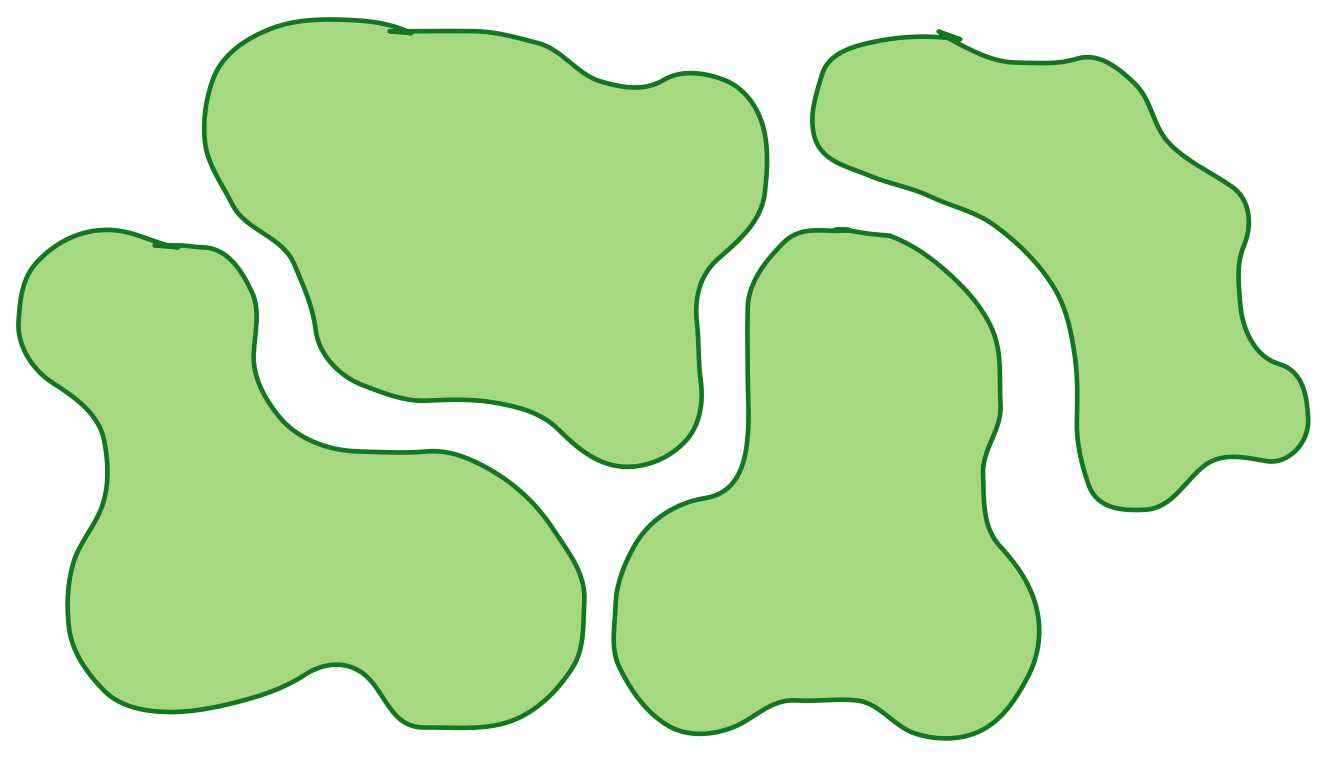
\includegraphics[width=2cm]{images/intro/objective_geom.png}};
						\node[title,font=\Large] at (1.6,0.1) {+};
						\node at (3.5,0.8) {Several Functions};
						\node[draw=none, inner sep=0pt] at (3.5,0) {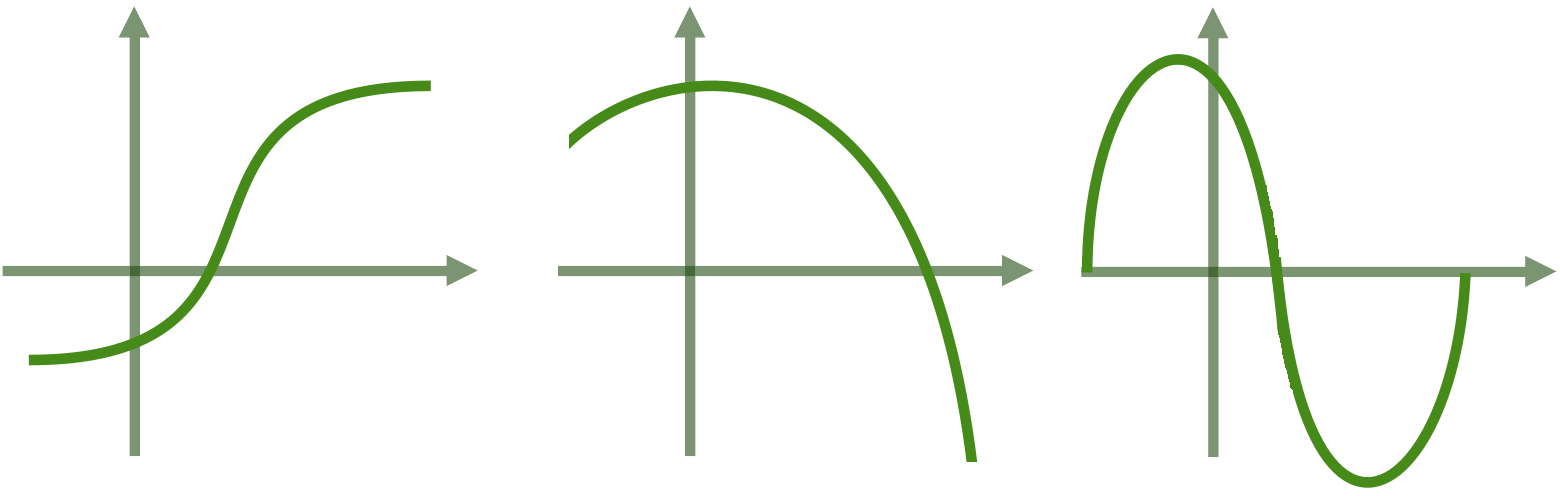
\includegraphics[width=3cm]{images/intro/objective_fct.png}};
						
						% Ajouter une flèche entre les deux rectangles
						\draw[->, title, line width=1.5pt] (5.5,0.1) -- (6.5,0.1);
						%		
						\node at (8,0.8) {Train a PINNs};
						\node[draw=none, inner sep=0pt] at (8,-0.1) {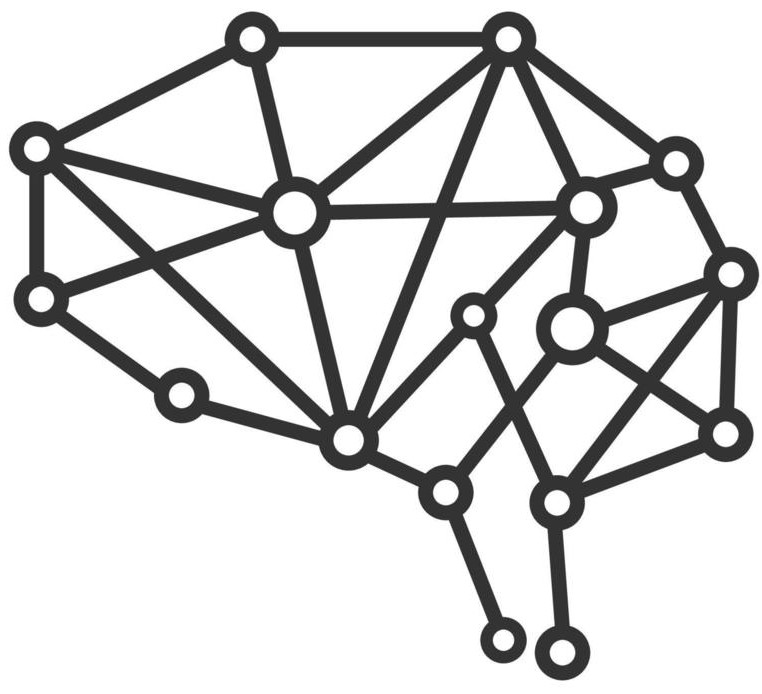
\includegraphics[width=1.5cm]{images/intro/objective_pinns.jpg}};				
					\end{tikzpicture}
				}%
			\end{figure}
			
			\textbf{ONLINE :}
			
			\vspace{-25pt}
			
			\begin{figure}[htb]
				\centering
				\resizebox{\textwidth}{!}{%
					\begin{tikzpicture}
						\node at (0,0.8) {1 Geometry - 1 Function};
						\node[draw=none, inner sep=0pt] at (0,0) {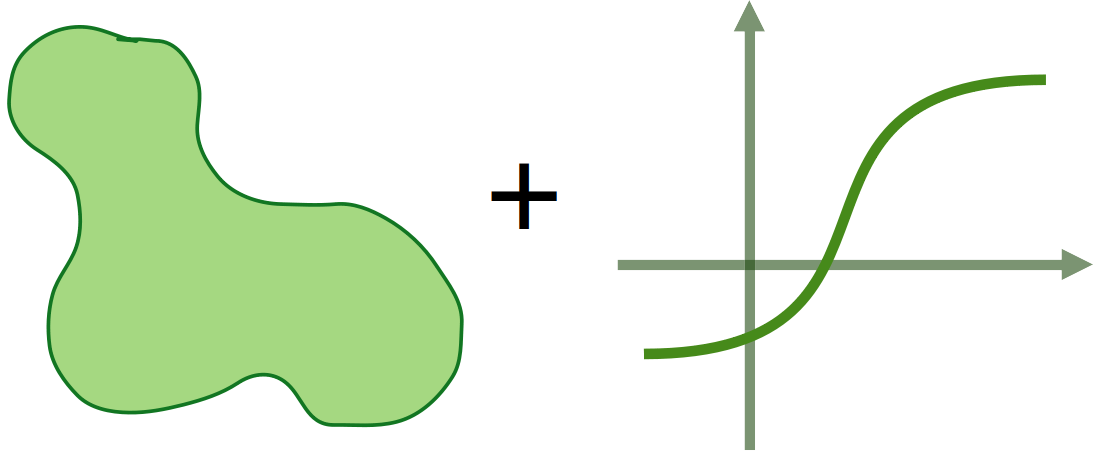
\includegraphics[width=2cm]{images/intro/objective_onegeom_onefct.png}};
						%		\node[title,font=\Large] at (1.6,0.1) {+};
						%		\node at (3.5,0.8) {Several Functions};
						%		\node[draw=none, inner sep=0pt] at (3.5,0) {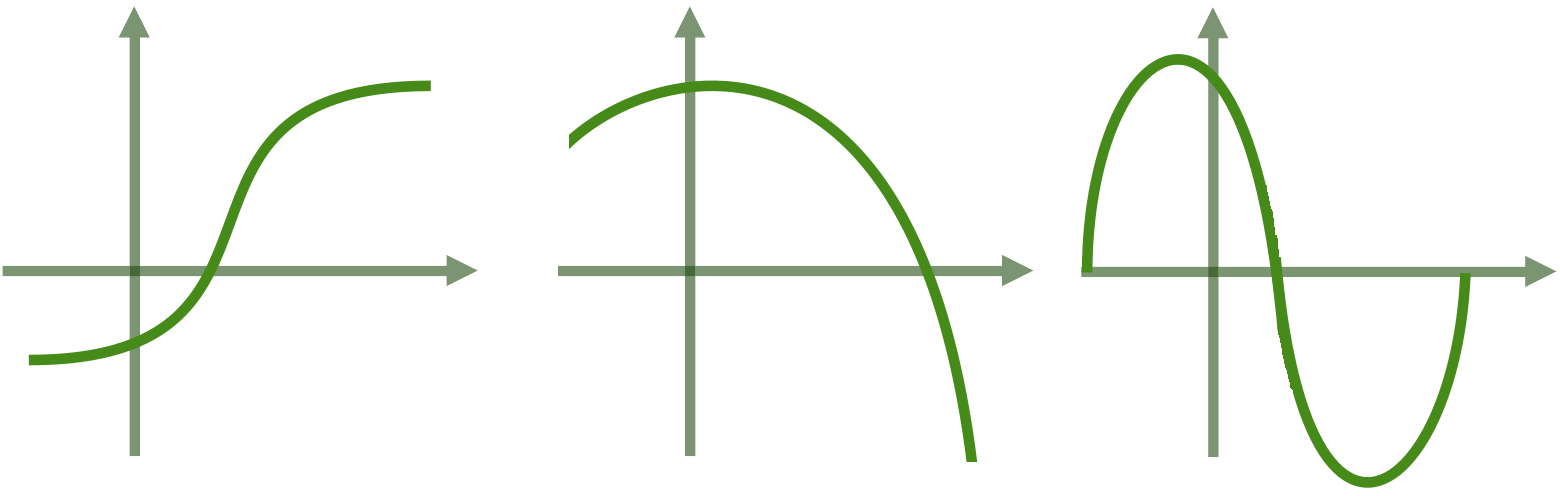
\includegraphics[width=3cm]{images/intro/objective_fct.png}};
						
						\draw[->, title, line width=1.5pt] (2,0.1) -- (3,0.1);
						
						\node[align=center] at (4,1) {Get PINNs \\ prediction};
						\node[draw=none, inner sep=0pt] at (4,-0.1) {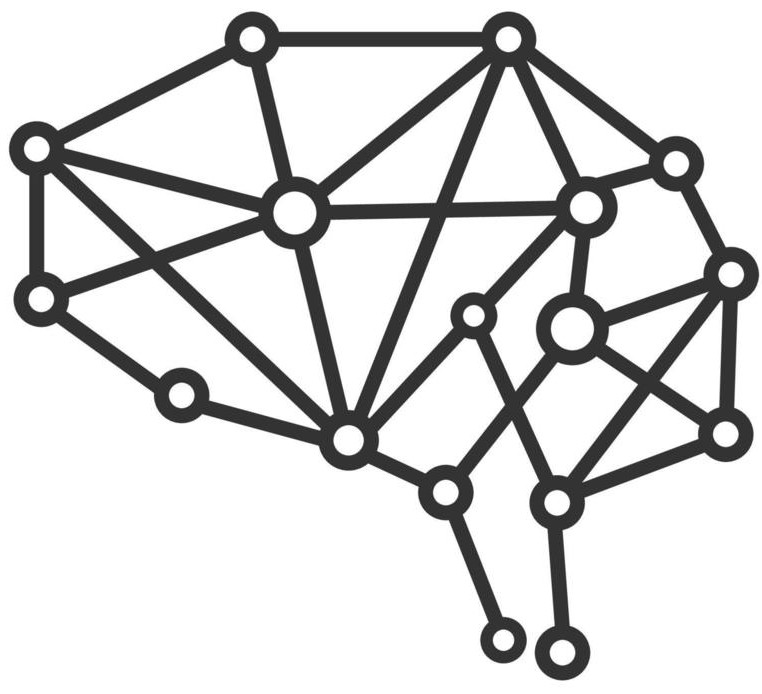
\includegraphics[width=1.5cm]{images/intro/objective_pinns.jpg}};
						
						% Ajouter une flèche entre les deux rectangles
						\draw[->, title, line width=1.5pt] (5.5,0.1) -- (6.5,0.1);
						%		
						\node[align=center] at (8,1) {Correct prediction \\ with $\phi$-FEM};
						\node[draw=none, inner sep=0pt] at (8,-0.1) {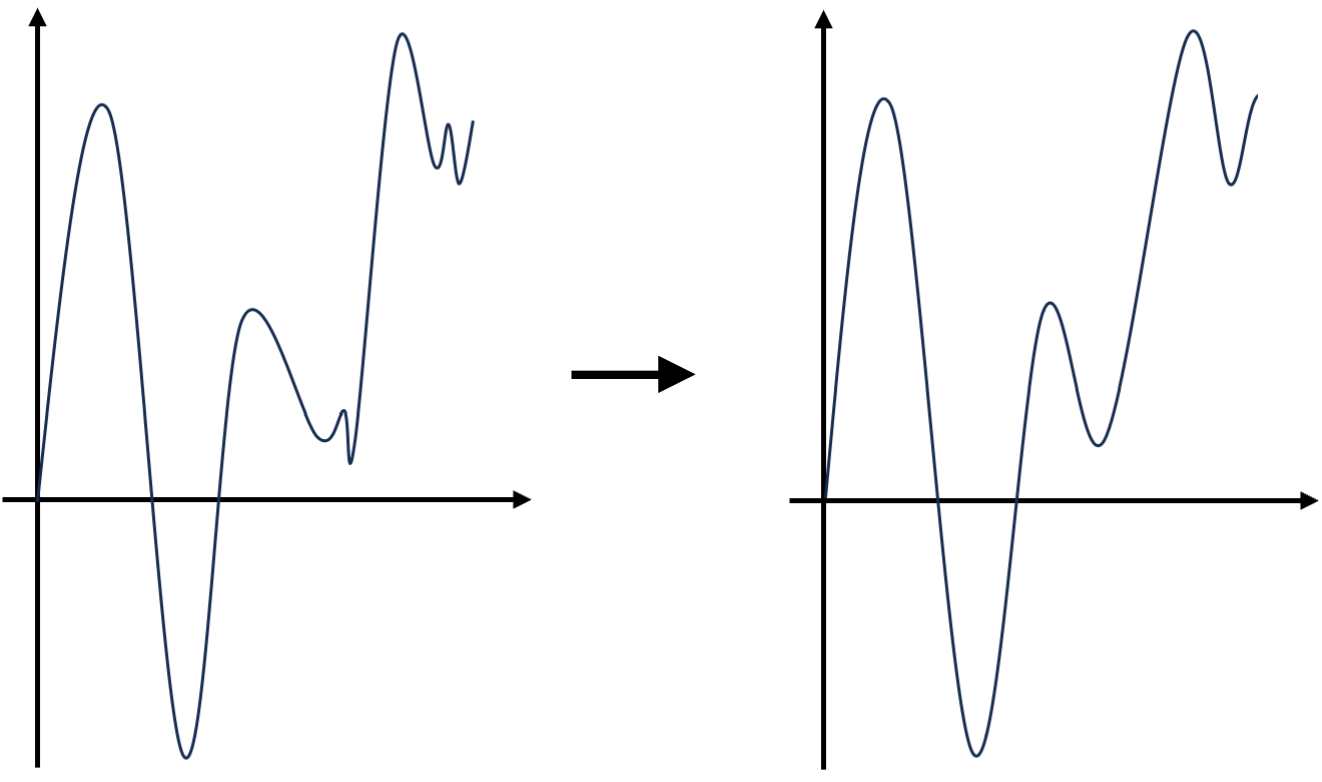
\includegraphics[width=2.5cm]{images/intro/objective_corr.png}};		
					\end{tikzpicture}
				}%
			\end{figure}
		\end{tcolorbox}
	\end{center}

    \textbf{Evolution :}

    \small
    % \setstretch{0.5}
    \begin{itemize}
        \item Geometry : 2D, simple, fixed (as circle, ellipse..) $ \; \rightarrow \;$ 3D / complex / variable
        \item PDE : simple, static (Poisson problem) $\; \rightarrow \;$ complex / dynamic (elasticity, hyper-elasticity)
        \item Neural Network : simple and defined everywhere (PINNs) $\; \rightarrow \;$ Neural Operator
    \end{itemize}
\end{frame}

\begin{frame}{Problem considered}
    \textbf{Elliptic problem with Dirichlet conditions :} \\
    Find $u : \Omega \rightarrow \mathbb{R}^d (d=1,2,3)$ such that
    \begin{equation}
    	\left\{\begin{aligned}
    		&L(u)=-\nabla \cdot (A(x) \nabla u(x)) + c(x)u(x) = f(x) \quad \text{in } \Omega, \\
    		&u(x) = g(x) \quad \text{on } \partial \Omega
    	\end{aligned}\right. \label{edp}
    \end{equation}
	with $A$ a definite positive coercivity condition and $c$ a scalar. We consider $\Delta$ the Laplace operator, $\Omega$ a smooth bounded open set and $\Gamma$ its boundary. 
    
    \textbf{Weak formulation :}
    \begin{equation*}
    	\text{Find } u\in V \text{ such that } a(u, v) = l (v) \forall v\in V
    \end{equation*}
    
    with
    \begin{align*}
    	a(u,v)&=\int_{\Omega} (A(x)\nabla u(x)) \cdot \nabla v(x) + c(x)u(x)v(x) \, dx \\
    	l(v)&=\int_{\Omega} f(x)v(x) \, dx
    \end{align*}
    
    \footnotesize
    \textit{Remark :} For simplicity, we will not consider 1st order terms. 

%    We will define by
%    \begin{equation*}
%        ||u_{ex}-u_{method}||_{0,\Omega}^{(rel)}=\frac{\int_\Omega (u_{ex}-u_{method})^2}{\int_\Omega u_{ex}^2}
%    \end{equation*}
%    the relative error between
%    \begin{itemize}
%        \item $u_{ex}$ : the exact solution  
%        \item $u_{method}$ : the solution obtained by a method \\
%        (can be : FEM or $\phi$-FEM, a correction solver or the prediction of an neural network).
%    \end{itemize}
\end{frame}

\begin{frame}{Numerical methods}
	\textbf{Objective :} Show that the philosophy behind most ofd the methods are the same.
	\begin{center}
		Mesh-based methods \hspace{5pt} // \hspace{5pt} Physically informed learning
	\end{center}
	
	\textbf{Numerical methods :} Discrete an infinite-dimensional problem (unknown = function) and solve it in a finite-dimensional space (unknown = vector).
	\begin{enumerate}[\textbullet]
		\item \textbf{Encoding :} we encode the problem in a finite-dimensional space
		\item \textbf{Approximation :} solve the problem in finite-dimensional space
		\item \textbf{Decoding :} bring the solution back into infinite dimensional space
	\end{enumerate}
	
	\begin{center}
		\begin{tabular}{|c|c|c|}
			\hline
			\textbf{Encoding} & \textbf{Approximation} & \textbf{Decoding} \\
			\hline
			$f \; \rightarrow \theta_f$ & $\theta_f \; \rightarrow \theta_u$ & $\theta_u \; \rightarrow u_\theta$ \\
			\hline
		\end{tabular}
	\end{center}
\end{frame}


	
	\renewcommand{\insertsectionheadSubtitle}{The PINN is parametrized by the $\bm{\mu}$ parameter.}
	\section[Parametric PINN]{Parametric Physics-Informed Neural Network (PINN)}
	\begin{frame}{Neural Network considered}
    \vspace{-2pt}
    We consider a parametric NN with 4 inputs and 4 outputs, defined by
    $$U_\theta(\bm{x},\bm{\mu}) = \big(u_{1,\theta},u_{2,\theta},p_\theta,T_\theta)(\bm{x},\bm{\mu}).$$
    
    The Dirichlet boundary conditions are imposed on the outputs of the MLP by a \textbf{post-processing} step. \citep{Sukumar_2022}
    
    \begin{center}
        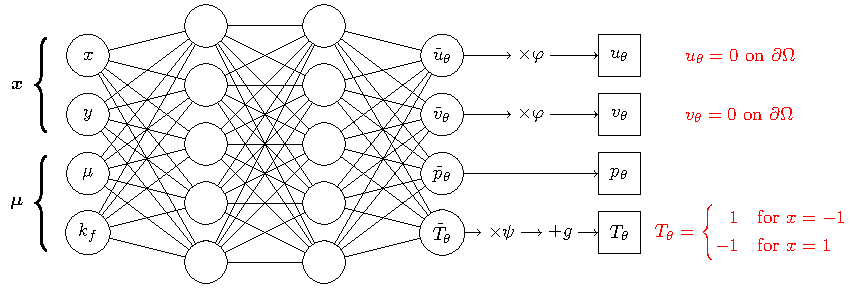
\includegraphics[width=0.85\linewidth]{images/pinn/network/network.pdf}
    \end{center}

    \vspace{-5pt}
    We consider two levelsets functions $\varphi_1$ and $\varphi_2$, and the linear function $g$ defined by
    \begin{equation*}
        \varphi_1(x,y) = (x-1)(x+1)(y-1)(y+1),
    \end{equation*}
    \begin{equation*}
        \varphi_2(x,y) = (x-1)(x+1) \quad \text{and} \quad g(x,y) = 1 - (x+1).
    \end{equation*}
\end{frame}

\begin{frame}{PINN training}
    \vspace{-4pt}
    \textbf{Approximate the solution of \eqref{eq:Pb} by a PINN :} Find the optimal weights $\theta^\star$, such that
	
    \vspace{-8pt}
    \begin{equation}
		\label{eq:opt_pb}
		\theta^\star = \argmin_{\theta}	\big( \; \textcolor{orange}{J_{inc}(\theta)} + \textcolor{orange}{J_{mom}(\theta)} + \textcolor{orange}{J_{ener}(\theta)} + \textcolor{darkred}{J_{ad}(\theta)} \; \big),
		\tag{$\mathcal{P}_\theta$}
	\end{equation}

    \vspace{-2pt}
	where the different cost functions\footnote[frame,1]{Discretized by a random process using Monte-Carlo method.} are defined by
	\vspace{5pt}

	\begin{minipage}{0.24\linewidth}
		\centering
		\textcolor{darkred}{adiabatic condition}
        
		\vspace{12pt}
		\textcolor{orange}{$3$ residual losses}
	\end{minipage}
	\begin{minipage}{0.68\linewidth}
		\centering
        \fcolorbox{darkred}{white}{
            $J_{ad}(\theta) =
            \int_{\mathcal{M}}\int_{\Gamma_\text{ad}} \big| \frac{\partial T_\theta(\bm{x},\bm{\mu})}{\partial n} \big|^2 d\bm{x} d\bm{\mu},$}
        
        \vspace{3pt}
		\fcolorbox{orange}{white}{
            $J_{\textbullet}(\theta) =
                \int_{\mathcal{M}}\int_{\Omega}
                \big| R_{\textbullet}(U_\theta(\bm{x},\bm{\mu});\bm{x},\bm{\mu}) \big|^2 d\bm{x} d\bm{\mu},$}
	\end{minipage}
    
    \vspace{5pt}
    with $U_\theta$ the parametric NN and $\textbullet$ the PDE considered (i.e. $inc$, $mom$ or $ener$).

    %\footnote[frame,2]{We consider a MLP with 5 hidden layers ($40,60,60,60,40$) and a 'sine' activation function. We train the PINN over $10000$ epochs ($3000$ ADAM / $7000$ LBFGS) with $40000$ collocation points in $\Omega$ and $30000$ points on the boundary $\partial\Omega\vert_{y=\pm 1}$.}
    
    \vspace{-7pt}
    \vspace{3pt}    
    \begin{center}
        \begin{minipage}{0.62\linewidth}
            \centering
            \vspace{-8pt}
            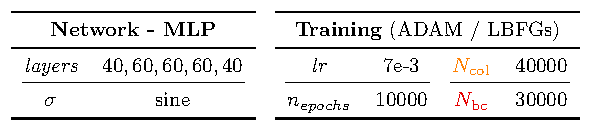
\includegraphics[width=0.94\linewidth]{images/pinn/training_param/training_param.pdf}
        \end{minipage}
        \begin{minipage}{0.36\linewidth}
            \centering
            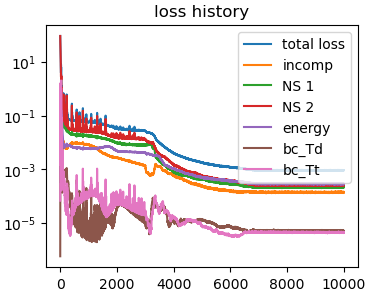
\includegraphics[width=0.84\linewidth]{images/pinn/training/test4_v5.png}
        \end{minipage}
    \end{center}
    
    \vspace{-8pt}
\end{frame}

\begin{frame}{Prediction on $\bm{\mu}^{(1)} = (0.1,0.1)$}
    \vspace{-4pt}
    \textbf{Prediction :} \begin{minipage}{0.26\linewidth}
        \centering
        $u_{1,\theta}$ \\
        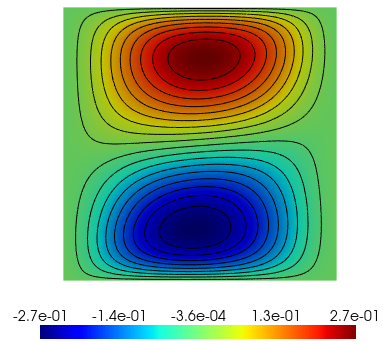
\includegraphics[width=0.95\linewidth]{images/pinn/training/PINN_plot_case4_v2_param1_u1.png}
    \end{minipage} \; \begin{minipage}{0.26\linewidth}
        \centering
        $u_{2,\theta}$ \\
        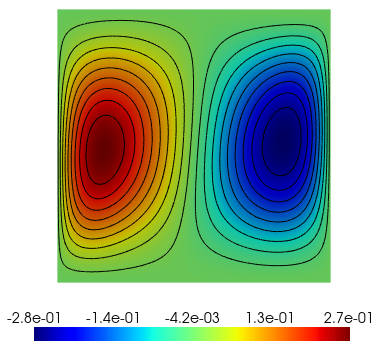
\includegraphics[width=0.95\linewidth]{images/pinn/training/PINN_plot_case4_v2_param1_u2.png}
    \end{minipage} \; \begin{minipage}{0.26\linewidth}
        \centering
        $T_\theta$ \\
        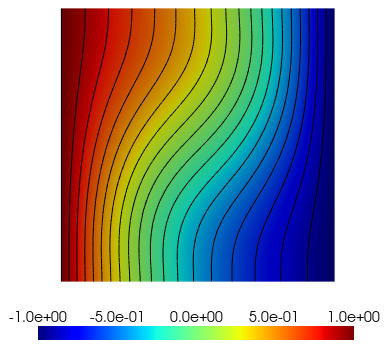
\includegraphics[width=0.95\linewidth]{images/pinn/training/PINN_plot_case4_v2_param1_T.png}
    \end{minipage}

    \vspace{8pt}

    \textbf{Error map :} \begin{minipage}{0.26\linewidth}
        \centering
        $u_{1,\text{ref}}-u_{1,\theta}$ \\
        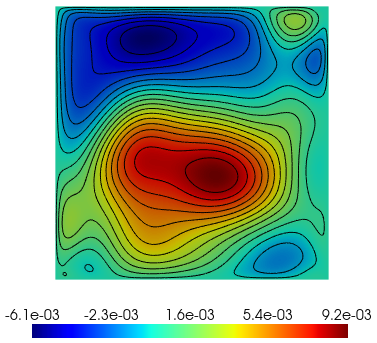
\includegraphics[width=0.95\linewidth]{images/pinn/training/PINN_error_plot_case4_v2_param1_u1.png}
    \end{minipage} \; \begin{minipage}{0.26\linewidth}
        \centering
        $u_{2,\text{ref}}-u_{2,\theta}$ \\
        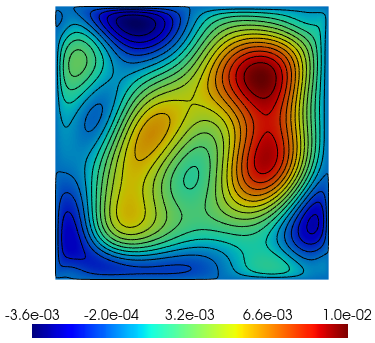
\includegraphics[width=0.95\linewidth]{images/pinn/training/PINN_error_plot_case4_v2_param1_u2.png}
    \end{minipage} \; \begin{minipage}{0.26\linewidth}
        \centering
        $T_\text{ref}-T_\theta$ \\
        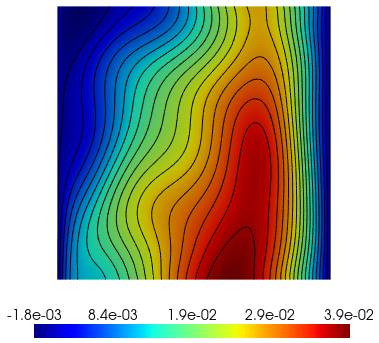
\includegraphics[width=0.95\linewidth]{images/pinn/training/PINN_error_plot_case4_v2_param1_T.png}
    \end{minipage}

    \vspace{8pt}

    \textbf{$L^2$ error :} \hspace{25pt} $2.98\times10^{-2} \hspace{42pt} 3.17\times10^{-2} \hspace{42pt}  3.90\times10^{-2}$

    \vspace{-2pt}
    \textbf{\small (relative)}
\end{frame}
	\renewcommand{\insertsectionheadSubtitle}{}

	\renewcommand{\insertsectionheadSubtitle}{The $\bm{\mu}$ parameter is fixed in the FE resolution.}
	\section{Finite element method (FEM)}
	\begin{frame}{Discrete weak formulation}
	\vspace{-2pt}
	We consider a mixed finite element space \; \fcolorbox{darkred}{white}{$M_h = [V_h^{\, 0}]^2 \times Q_h \times W_h$} \; and
	
	\vspace{-4pt}
	\begin{center}
		\begin{tabular}{ccccccccl}
		\uncover<0>{\footnotesize \big(dim$(V_h^{\, 0})=N_u$\big)} \qquad & $\bm{u}_h$ & $\in$ & $[V_h^{\, 0}]^2$ & $\subset$ & $[H^1_0(\Omega)]^2$ & : & $\mathbb{P}_2$ & \multirow{2}{*}{$\left. \rule{0pt}{1.7em} \right\} \;$ \footnotesize (Taylor–Hood spaces)} \\
		\uncover<0>{\footnotesize \big(dim$(Q_h)=N_p$\big)} \qquad & $p_h$ & $\in$ & $Q_h$ & $\subset$ & $L^2_0(\Omega)$ & : & $ \mathbb{P}_1$ & \\ 
		\uncover<0>{\footnotesize \big(dim$(W_h)=N_T$\big)} \qquad & $T_h$ & $\in$ & $W_h$ & $\subset$ & $W$ & : & $\mathbb{P}_2$ & 
		\end{tabular}
	\end{center}

	with $\;W = \{w\in H^1(\Omega), \; w\vert_{x=-1}=1, \; w\vert_{x=1}=-1\}$.

	\vspace{5pt}

	\textbf{Weak problem :} Find $U_h=(\bm{u}_h, p_h, T_h) \in M_h$ s.t., \; $\forall (\bm{v}_h, q_h, w_h) \in M_h^{\, 0} $,

	\vspace{-4pt}
	\footnotesize
	\begin{equation}
		\label{eq:weak_pb}
		\begin{aligned}
			&\int_\Omega (\bm{u}_h \cdot \nabla)\bm{u}_h \cdot \bm{v}_h \, d\bm{x} + \mu \int_\Omega \nabla \bm{u}_h : \nabla \bm{v}_h \, d\bm{x} \\
			&\hspace{50pt} - \int_\Omega p_h \, \nabla \cdot \bm{v}_h \, d\bm{x} - g \int_\Omega (1 + \beta T_h) \bm{e}_y \cdot \bm{v}_h \, d\bm{x} = 0, \qquad\text{\footnotesize (momentum)} \\
			&\int_\Omega q_h \, \nabla \cdot \bm{u}_h \, d\bm{x} \, + \, 10^{-4} \int_\Omega q_h \, p_h \, d\bm{x} = 0, \qquad\text{\footnotesize (incompressibility + pressure penalization)}\\
			&\int_\Omega (\bm{u}_h \cdot \nabla T_h) \, w_h \, d\bm{x} + \int_\Omega k_f \nabla T_h \cdot \nabla w_h \, d\bm{x} = 0,  \qquad\text{\footnotesize (energy)}
			% \epsilon \int_\Omega q \, p \, dx = 0
		\end{aligned}
		\tag{$\mathcal{P}_h$}
	\end{equation}
	
	\vspace{5pt}
	where $M_h^{\, 0} = [V_h^{\, 0}]^2 \times Q_h \times W_h^{\, 0}$ with $W_h^{\, 0} \subset \{w \in H^1[\Omega], \; w\vert_{x=\pm 1}=0\}$.
\end{frame}

\begin{frame}{Newton method}
	We consider the following three parameters:
	$$\bm{\mu}^{(1)} = (0.1,0.1), \; \bm{\mu}^{(2)} = (0.05,0.05) \; \text{and} \; \bm{\mu}^{(3)} = (0.01,0.01).$$

	Denoting $N_h$ the dimension of $M_h$, we want to solve the non linear system: %\hfill \footnotesize $N_h$ : dimension of $M_h$.

    \normalsize
    \vspace{-10pt}
    \begin{equation*}
        % \label{eq:nonlinear}
        F(\vec{U}_k) = 0 
    \end{equation*}

    with $F:\mathbb{R}^{N_h} \to \mathbb{R}^{N_h}$ a non linear operator and $\vec{U}_k\in \mathbb{R}^{N_h}$ the unknown vector associated to the $k$-th parameter $\bm{\mu}^{(k)}$ ($k=1,2,3$). \quad\refappendix{frame:basis}

	\setcounter{algocf}{0}
    \begin{center}
        \small
        \begin{minipage}{0.9\linewidth}
            \begin{algorithm}[H]
                \SetAlgoLined
                \caption{Newton algorithm} % \citep{newton_accel_2025}}
                \textbf{Initialization step:} set $\vec{U}_k^{(0)} = \only<1>{\vec{U}_{k,0}}\only<2>{\textcolor{darkred}{\vec{U}_{k,0}}}$\;
                \For{\( n \ge 0 \)}{
                    Solve the linear system \( F(\vec{U}_k^{(n)}) + F'(\vec{U}_k^{(n)}) \delta_k^{(n+1)} = 0 \) for \( \delta_k^{(n+1)} \)\;
                    Update \( \vec{U}_k^{(n+1)} = \vec{U}_k^{(n)} + \delta_k^{(n+1)} \)\;
                }
            \end{algorithm}
        \end{minipage}
    \end{center}
	\uncover<2>{\textcolor{darkred}{How to initialize the Newton solver?}}
\end{frame}

\begin{frame}{3 types of initialization}
	\begin{itemize}
		\item \textbf{Natural :} \only<2-4>{Using constant or linear function.}
		
		\only<2>{Considering a fixed parameter with $k\in\{1,2,3\}$, we can use the following initialization:	
		$$\vec{U}_{k,0} = \big(\vec{0}, \vec{0}, \vec{0}, \vec{T}_0\big)$$
		where for $i=1,\ldots,\text{dim}(W_h)$,
		$$(\vec{T}_0)_i = g(\bm{x}^{(i)}) = 1 - (x^{(i)}+1)$$
		with $\bm{x}^{(i)}=\big(x^{(i)},y^{(i)}\big)$ the $i$-th dofs coordinates of $W_h$.}
		
		\item \textbf{PINN :} \only<3-4>{Using PINN prediction. \\	
		(UNet : \citep{odot_deepphysics_2021} ; FNO : \citep{newton_accel_2025})} \\
		\only<3>{Considering a fixed parameter with $k\in\{1,2,3\}$, we can use the following initialization for $i=1,\ldots,N_h$,
		$$\big(\vec{U}_{k,0}\big)_i = U_\theta(\bm{x}^{(i)},\bm{\mu}^{(k)})$$
		with $\bm{x}^{(i)}=\big(x^{(i)},y^{(i)}\big)$ the $i$-th dofs coordinates of $M_h$ and $U_\theta$ the PINN.}
		
		\item \textbf{Continuation method :} \only<4>{Using a coarse FE solution of a simpler parameter.}
		
		\only<4>{\begin{itemize}
			\item We consider a fixed parameter with $k\in\{2,3\}$.
			\item We consider a coarse grid ($16\times 16$ grid) and compute the FE solution of \eqref{eq:weak_pb} for the parameter $\bm{\mu}^{(k-1)}$.
			\item We interpolate the coarse solution to the current mesh.
			\item We use it as an initialization for the Newton method, i.e.
			$$\vec{U}_{k,0} = \big(\vec{u}_{k-1}, \vec{v}_{k-1}, \vec{p}_{k-1}, \vec{T}_{k-1}\big)$$
			where $\vec{u}_{k-1}$, $\vec{v}_{k-1}$, $\vec{p}_{k-1}$ and $\vec{T}_{k-1}$ are the FE solutions for the parameter $\bm{\mu}^{(k-1)}$.
		\end{itemize}
		}
	\end{itemize}
\end{frame}
	\renewcommand{\insertsectionheadSubtitle}{}

	\section{Enriched finite element method using PINN}
	\subsection{Very simple linear test case}

\begin{frame}{What is the purpose of enrichment?}

\vspace{-5pt}
\only<1>{\textbf{Poisson problem} (with Dirichlet BC) \textbf{:} \; Find $u : \Omega \rightarrow \mathbb{R}$ such that
\vspace{-5pt}
\begin{equation*}
    \left\{
    \begin{aligned}
        -\Delta u & = f, \; &  & \text{in } \; \Omega, \\
        u         & =0, \;  &  & \text{on } \; \partial\Omega.
    \end{aligned}
    \right.
    % \label{eq:Lap2D}\tag{$\mathcal{P}$}
\end{equation*}}

\only<2>{\textbf{\textcolor{darkred}{Modified} Poisson problem :} \; Find $\textcolor{darkred}{C_{h,u}^+} : \Omega \rightarrow \mathbb{R}$ such that
\vspace{-5pt}
\begin{equation*}
    \left\{
    \begin{aligned}
        -\Delta \textcolor{darkred}{C_{h,u}^+} & = f + \textcolor{darkred}{\Delta u_\theta}, \; &  & \text{in } \; \Omega, \\
        \textcolor{darkred}{C_{h,u}^+} & =0, \;  &  & \text{on } \; \partial\Omega,
    \end{aligned}
    \right.
    % \label{eq:Lap2D}\tag{$\mathcal{P}$}
\end{equation*}
with $u_{\theta}$ a PINN prediction.}

\only<1>{\textbf{Variational Problem :} We consider $V_h^0$ a $\mathbb{P}_k$ continuous Lagrange FE space ($k\geq 1$).
\begin{equation}
    \label{eq:weakform}
    \text{Find } u_h\in V_h^0 \;\text{such that}, \forall v_h\in V_h^0, a(u_h,v_h)=l(v_h),
    \tag{$\mathcal{P}_h$}
\end{equation}
\vspace{1pt}
with $h$ the characteristic mesh size, $a$ and $l$ the associated bilinear and linear forms.}

\only<2-3>{\textbf{\textcolor<2>{darkred}{Modified} variational Problem :} 
\begin{equation}
    \label<2>{eq:weakplus}
    \text{Find } \textcolor<2>{darkred}{C_{h,u}^+} \in V_h^0 \text{ such that}, \forall v_h \in V_h^0, a(\textcolor<2>{darkred}{C_{h,u}^+},v_h) = l(v_h) \textcolor<2>{darkred}{- a(u_{\theta},v_h)},\tag{$\mathcal{P}_h^+$}
\end{equation}
with the \textcolor<2>{darkred}{enriched trial space $V_h^+$} defined by
\begin{equation*}
    V_h^+ = \left\{
    \textcolor<3>{darkred}{u_h^+= u_{\theta} + C_{h,u}^+}, \quad C_{h,u}^+ \in V_h^0
    \right\}.
\end{equation*}}

\vspace{-5pt}
\only<3>{
    \begin{center}
        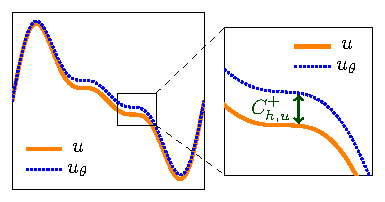
\includegraphics[width=0.6\linewidth]{images/efup/correction_entier/correction.pdf}
    \end{center}
}

\vspace{-8pt}
\only<3>{\begin{center}
    \textcolor{darkred}{\textbf{We hope that the modified problem will give the same results \\
    as the standard one on coarser meshes.}}
\end{center}
}

\end{frame}

\begin{frame}{Convergence analysis}
	\vspace{-10pt}
	\hypersetup{
		citecolor=white,
	}

	\begin{mytheo}{Convergence analysis of the standard FEM \footnotesize\citep{Ern2004TheoryAP}\normalsize}{fem}
		We denote $u_h\in V_h$ the solution of \eqref{eq:weakform} with $V_h$ the standard trial space. Then,
		\vspace{-5pt}
		\begin{equation*}
			| u-u_h|_{H^1} \leqslant C_{H^1} \, h^{k} |u|_{H^{k+1}},
		\end{equation*}
		\begin{equation*}
			\| u-u_h\|_{L^2} \leqslant C_{L^2} \, h^{k+1} |u|_{H^{k+1}}.
		\end{equation*}
	\end{mytheo}
	
	\begin{mytheo}{Convergence analysis of the enriched FEM \footnotesize\citep{ours_2025}\normalsize}{add}
		We denote $u_h^+\in V_h^+$ the solution of \eqref{eq:weakplus} with $V_h^+$ the enriched trial space. Then,
		\vspace{-5pt}
		\begin{equation*}
			| u-u_h^+|_{H^1} \leqslant \fcolorbox{orange}{other!10!white}{$\frac{| u-u_{\theta} |_{H^{k+1}}}{| u |_{H^{k+1}}}$} \left(C_{H^1} \, h^{k} |u|_{H^{k+1}}\right),
		\end{equation*}
		\begin{equation*}
			\| u-u_h^+\|_{L^2} \leqslant \fcolorbox{orange}{other!10!white}{$\frac{| u-u_{\theta} |_{H^{k+1}}}{| u |_{H^{k+1}}}$} \left(C_{L^2} \, h^{k+1} |u|_{H^{k+1}}\right).
		\end{equation*}
	\end{mytheo}

	\hypersetup{
		citecolor=other,
	}

	\footnotesize
	\textcolor{orange}{Gains of the additive approach.}
\end{frame}


\subsection{The heated cavity test case considered}

\begin{frame}{Enriched space using PINN} %\footnote[frame,1]{The $\bm{\mu}$ parameter is fixed in the FE resolution.}}	
    Considering the PINN prior $U_\theta = (\bm{u}_\theta, p_\theta, T_\theta)$, we define the \textcolor{darkred}{mixed finite element space additively enriched} by the PINN as follows:
    
    \begin{center}
        \fcolorbox{darkred}{white}{$M_h^+ = \left\{U_h^+ = U_\theta + C_h^+, \quad C_h^+ \in M_h^{\, 0}\right\}$}
    \end{center}

    with $M_h^{\, 0}=[V_h^{\, 0}]^2 \times Q_h \times W_h^0$,
    $U_h^+ = (\bm{u}_h^+, p_h^+, T_h^+) \in M_h^+$ and $C_h^+ = (\bm{C}_{h,\bm{u}}^+, C_{h,p}^+, C_{h,T}^+)$.

    \vspace{8pt}

    We can then define the three finite element subspaces of $M_h^+$ as follows:
    \begin{minipage}{0.6\linewidth}
        \vspace{-15pt}
        \begin{align*}
            \bm{V}_h^+ &= \left\{\bm{u}_h^+ = \bm{u}_\theta + \bm{C}_{h,\bm{u}}^+, \; \bm{C}_{h,\bm{u}}^+ \in [V_h^{\, 0}]^2\right\}, \\
            Q_h^+ &= \left\{p_h^+ = p_\theta + C_{h,p}^+, \; C_{h,p}^+ \in Q_h\right\}, \\
            W_h^+ &= \left\{T_h^+ = T_\theta + C_{h,T}^+, \; C_{h,T}^+ \in W_h^{\, 0}\right\},
        \end{align*}
        where $\bm{C}_{h,\bm{u}}^+$, $C_{h,p}^+$ and $C_{h,T}^+$ becomes the unknowns.
        
        % \vspace{5pt}
        % \hl{à ajouter : dans quoi vit $U_\theta$ ?}
    \end{minipage}
    \begin{minipage}{0.38\linewidth}
        \centering
        \vspace{5pt}
        \pgfimage[width=0.7\linewidth]{images/efup/correction/correction.pdf}
    \end{minipage}
\end{frame}


\begin{frame}{Weak formulation - Additive approach}
    \textbf{Weak problem :} Find $C_h^+=(\textcolor{Cyan}{\bm{C}_{h,\bm{u}}^+}, \textcolor{blue}{C_{h,p}^+}, \textcolor{ForestGreen}{C_{h,T}^+}) \in M_h^{\, 0}$ s.t., \; $\forall (\bm{v}_h, q_h, w_h) \in M_h^{\, 0}$,

    \vspace{-4pt}
    \footnotesize
    \begin{equation}
        \label{eq:weak_pb_add}
        \hspace{-8pt}\begin{aligned}
            &\int_\Omega \big[(\textcolor{darkred}{\bm{u}_\theta} \cdot \nabla)\textcolor{darkred}{\bm{u}_\theta} + (\textcolor{darkred}{\bm{u}_\theta} \cdot \nabla)\textcolor{Cyan}{\bm{C}_{h,\bm{u}}^+} + (\textcolor{Cyan}{\bm{C}_{h,\bm{u}}^+} \cdot \nabla)\textcolor{darkred}{\bm{u}_\theta} + (\textcolor{Cyan}{\bm{C}_{h,\bm{u}}^+} \cdot \nabla)\textcolor{Cyan}{\bm{C}_{h,\bm{u}}^+} \big] \cdot \bm{v_h} \, d\bm{x} \\
            &\hspace{20pt} +\mu \left(\int_\Omega  \nabla \textcolor{darkred}{\bm{u}_\theta} : \nabla \bm{v}_h \, d\bm{x} + \int_\Omega \nabla \textcolor{Cyan}{\bm{C}_{h,\bm{u}}^+} : \nabla \bm{v}_h \, d\bm{x}\right) + \left(\int_\Omega \nabla \textcolor{darkred}{p_\theta} \cdot \bm{v}_h \, d\bm{x} - \int_\Omega \textcolor{blue}{C_{h,p}^+} \nabla \cdot \bm{v}_h \, d\bm{x}\right)\\
            &\hspace{50pt} - g \int_\Omega (1 + \beta (\textcolor{darkred}{T_\theta} + \textcolor{ForestGreen}{C_{h,T}^+})) \bm{e}_y \cdot \bm{v}_h \, d\bm{x} = 0, \,\text{\footnotesize (momentum)}  \\
            &\int_\Omega q_h \, \big[\nabla \cdot \textcolor{darkred}{\bm{u}_\theta} + \nabla \cdot \textcolor{Cyan}{\bm{C}_{h,\bm{u}}^+}\big] \, d\bm{x} \, + \, 10^{-4} \int_\Omega q_h \, (\textcolor{darkred}{p_\theta} + \textcolor{blue}{C_{h,p}^+}) \, d\bm{x} = 0, \; \text{\footnotesize (incompressibility + penal)} \\
            & \int_\Omega \big[ \textcolor{darkred}{\bm{u}_\theta} \cdot \nabla \textcolor{darkred}{T_\theta} + \textcolor{darkred}{\bm{u}_\theta} \cdot \nabla \textcolor{ForestGreen}{C_{h,T}^+} + \textcolor{Cyan}{\bm{C}_{h,\bm{u}}^+} \cdot \nabla \textcolor{darkred}{T_\theta} + \textcolor{Cyan}{\bm{C}_{h,\bm{u}}^+} \cdot \nabla \textcolor{ForestGreen}{C_{h,T}^+} \big] w_h \, d\bm{x} \\
            & \hspace{40pt} + k_f \left(\int_\Omega \nabla \textcolor{darkred}{T_\theta} \cdot \nabla w_h \; d\bm{x} + \int_\Omega \nabla \textcolor{ForestGreen}{C_{h,T}^+} \cdot \nabla w_h \, d\bm{x} \, w_h \, d\bm{s}\right) = 0, \, \text{\footnotesize (energy)}
        \end{aligned}
        \tag{$\mathcal{P}_h^+$}
    \end{equation}

    \vspace{5pt}
    with \textcolor{darkred}{$U_\theta = (\bm{u}_\theta, p_\theta, T_\theta)$} the PINN prior and some modified boundary conditions.
\end{frame}

\begin{frame}{Newton method - Additive approach}
    \vspace{-5pt}
    We want to solve the non linear system: %\hfill \tiny $N_h$ : number of degrees of freedom.

    \normalsize
    \vspace{-10pt}
    \begin{equation*}
        % \label{eq:nonlinear}
        F_\theta(\vec{C}) = 0 
    \end{equation*}

    \vspace{-2pt}
    with $F_\theta:\mathbb{R}^{N_h} \to \mathbb{R}^{N_h}$ the non linear operator associated to the weak problem \eqref{eq:weak_pb_add} and $\vec{C}\in \mathbb{R}^{N_h}$ the \textcolor{darkred}{correction vector (unknown)}.

	\setcounter{algocf}{1}
    \begin{center}
        \small
        \begin{minipage}{0.9\linewidth}
            \begin{algorithm}[H]
                \SetAlgoLined
                \caption{Newton algorithm \citep{newton_accel_2025}}
                \textbf{Initialization step:} set $\vec{C}^{(0)} = \textcolor{darkred}{0}$\;
                \For{\( n \ge 0 \)}{
                    Solve the linear system \( F_\theta(\vec{C}^{(n)}) + F_\theta'(\vec{C}^{(n)}) \delta^{(n+1)} = 0 \) for \( \delta^{(n+1)} \)\;
                    Update \( \vec{C}^{(n+1)} = \vec{C}^{(n)} + \delta^{(n+1)} \)\;
                }
            \end{algorithm}
        \end{minipage}
    \end{center}
    
    \vspace{3pt}
    \textbf{Advantage compared to PINN initialization\footnote[frame,1]{Taking $U_\theta$ and $C_h^+$ in the same space, additive approach is exactly the same as the PINN initialization.}:} %\refappendix{frame:comp}

    \vspace{-2pt}
    \begin{center}
        \textcolor{darkred}{$u_\theta$ is not required to live in the same discrete space as $C_h^+$}.
    \end{center}
    \vspace{8pt}
\end{frame}
	% \subsection{Additive approach}

\begin{frame}{Additive approach}
	\textbf{Variational Problem :} Let $u_{\theta} \in H^{k+1}(\Omega)\cap H^1_0(\Omega)$.
	
	\vspace{-5pt}
	\begin{equation}
		\label{eq:weakplus}
		\text{Find } p_h^+ \in V_h^0 \text{ such that}, \forall v_h \in V_h^0, a(p_h^+,v_h) = l(v_h) - a(u_{\theta},v_h),\tag{$\mathcal{P}_h^+$}
	\end{equation}
	
	\vspace{5pt}
	\begin{minipage}[t]{0.6\linewidth}
		with the \textcolor{red}{enriched trial space $V_h^+$} defined by
		\begin{equation*}
			V_h^+ = \left\{
			u_h^+= u_{\theta} + p_h^+, \quad p_h^+ \in V_h^0
			\right\}.
		\end{equation*}
	
		\vspace{20pt}
	
		\textbf{General Dirichlet BC :} If $u=g$ on $\partial \Omega$, then
		\[
			p_h^+ = g - u_{\theta} \text{\quad on } \partial \Omega,
		\]
		with $u_\theta$ the PINN prior. 
	\end{minipage} \qquad \begin{minipage}[t][][b]{0.28\linewidth}
		\vspace{-15pt}
		\centering
		\pgfimage[width=\linewidth]{images/correction/correction.pdf}
	\end{minipage}
\end{frame}

\begin{frame}{Convergence analysis}
	\vspace{-10pt}
	\hypersetup{
		citecolor=white,
	}

	\begin{mytheo}{Convergence analysis of the standard FEM \footnotesize\citep{Ern2004TheoryAP}\normalsize}{fem}
		We denote $u_h\in V_h$ the solution of \eqref{eq:weakform} with $V_h$ the standard trial space. Then,
		\vspace{-5pt}
		\begin{equation*}
			| u-u_h|_{H^1} \leqslant C_{H^1} \, h^{k} |u|_{H^{k+1}},
		\end{equation*}
		\begin{equation*}
			\| u-u_h\|_{L^2} \leqslant C_{L^2} \, h^{k+1} |u|_{H^{k+1}}.
		\end{equation*}
	\end{mytheo}
	
	\begin{mytheo}{Convergence analysis of the enriched FEM \footnotesize\citep{ours_2025}\normalsize}{add}
		We denote $u_h^+\in V_h^+$ the solution of \eqref{eq:weakplus} with $V_h^+$ the enriched trial space. Then,
		\vspace{-5pt}
		\begin{equation*}
			| u-u_h^+|_{H^1} \leqslant \fcolorbox{orange}{other!10!white}{$\frac{| u-u_{\theta} |_{H^{k+1}}}{| u |_{H^{k+1}}}$} \left(C_{H^1} \, h^{k} |u|_{H^{k+1}}\right),
		\end{equation*}
		\begin{equation*}
			\| u-u_h^+\|_{L^2} \leqslant \fcolorbox{orange}{other!10!white}{$\frac{| u-u_{\theta} |_{H^{k+1}}}{| u |_{H^{k+1}}}$} \left(C_{L^2} \, h^{k+1} |u|_{H^{k+1}}\right).
		\end{equation*}
	\end{mytheo}

	\hypersetup{
		citecolor=other,
	}

	\footnotesize
	\textcolor{orange}{Gains of the additive approach.}
\end{frame}

\subsection{Numerical results \filledstar}

\begin{frame}{1st problem considered} 
	\textbf{Problem statement:} Considering an \textcolor{red}{Anisotropic Elliptic problem with Dirichlet BC}:
	\vspace{-5pt}
	\begin{equation*}
		\left\{
		\begin{aligned}
			-\text{div}(D\nabla u) & = f, \; &  & \text{in } \; \Omega, \\
			u         & =0, \;  &  & \text{on } \; \partial\Omega,
		\end{aligned}
		\right.
		% \label{eq:Ell2D}\tag{$\mathcal{P}$}
	\end{equation*}

	with $\Omega=[0,1]^2$ and $\mathcal{M}=[0.4, 0.6]\times [0.4, 0.6]\times [0.01,1]\times [0.1,0.8]$ ($p=4$).
	
	\vspace{8pt}
	\textbf{Right-hand side :}

	\vspace{-5pt}
	\begin{equation*}
		f(\bm{x},\bm{\mu})=\exp\left(-\frac{(x-\mu_1)^2+(y-\mu_2)^2}{0.025\sigma^2}\right).
	\end{equation*}
	
	\textbf{Diffusion matrix :} (symmetric and positive definite)
	\begin{equation*}
		D(\bm{x},\bm{\mu})=\begin{pmatrix}
			\epsilon x^2+y^2 & (\epsilon-1)xy \\
			(\epsilon-1)xy & x^2+\epsilon y^2
		\end{pmatrix}.
	\end{equation*}

	\vspace{2pt}
	\small
	\textbf{PINN training:} Imposing BC exactly with a level-set function.
\end{frame}

\begin{frame}{Numerical results}
	\hspace{-5pt}\begin{minipage}[t]{0.46\linewidth}
		\textbf{Error estimates :} 1 set of parameters.
		$$\bm{\mu}^{(1)}=(0.51,0.54,0.52,0.55)$$
		\vspace{-35pt}
		\begin{figure}[H]
			\cvgFEMCorrAlldeg{images/numeric/elliptic/cvg/FEM_case3_v1_param1.csv}{images/numeric/elliptic/cvg/Corr_case3_v1_param1.csv}{1e-9}
		\end{figure}
	\end{minipage} \qquad \small
	\begin{minipage}[t]{0.48\linewidth}
	\end{minipage}
\end{frame}

\begin{frame}[noframenumbering]{Numerical results}
	\hspace{-5pt}\begin{minipage}[t]{0.46\linewidth}
		\textbf{Error estimates :} 1 set of parameters.
		$$\bm{\mu}^{(1)}=(0.51,0.54,0.52,0.55)$$
		\vspace{-35pt}
		\begin{figure}[H]
			\cvgFEMCorrAlldeg{images/numeric/elliptic/cvg/FEM_case3_v1_param1.csv}{images/numeric/elliptic/cvg/Corr_case3_v1_param1.csv}{1e-9}
		\end{figure}
	\end{minipage} \qquad \small
	\begin{minipage}[t]{0.48\linewidth}
		\textbf{Gains achieved :} $n_p=50$ sets of parameters.
		$$\mathcal{S}=\left\{\bm{\mu}^{(1)},\dots,\bm{\mu}^{(n_p)}\right\}$$
		\vspace{-15pt}
		\begin{table}[H]
			\gainstableallq{images/numeric/elliptic/gains/Tab_stats_case3_v1.csv}
		\end{table}

		\normalsize\centering\vspace{-20pt}
		$$N=20$$

		\vspace{-5pt}
		Gain : $\| u-u_h\|_{L^2} / \| u-u_h^+\|_{L^2}$ \\
		
		\small\vspace{8pt}
		Cartesian mesh : $N^2$ nodes.
	\end{minipage}
\end{frame}

\begin{frame}{Numerical solutions}
	\begin{figure}[!ht] \centering
		\includegraphics[width=0.33\linewidth]{images/numeric/elliptic/plots/standalone_solutions_cropped.pdf}		
		\includegraphics[width=0.7\linewidth]{images/numeric/elliptic/plots/standalone_errors.pdf}
	\end{figure}

	\vspace{-8pt}
	$$\bm{\mu}^{(2)}=(0.46,0.52,0.05,0.12)$$
\end{frame}

\begin{frame}{2nd problem considered} 
	\textbf{Problem statement:} Considering the \textcolor{red}{Poisson problem with mixed BC}:
	\vspace{-5pt}
	\begin{equation*}
		\left\{
		\begin{aligned}
			-\Delta u & = f, \; &  & \text{in } \; \Omega \times \mathcal{M}, \\
			u         & = g, \;  &  & \text{on } \; \Gamma_E \times \mathcal{M}, \\
			\smash{\frac{\partial u}{\partial n}}+u  & = g_R, \;  &  & \text{on } \; \Gamma_I \times \mathcal{M},
		\end{aligned}
		\right.
		% \label{eq:Lap2DMixed}\tag{$\mathcal{P}$}
	\end{equation*}

	with $\Omega=\{(x,y)\in\mathbb{R}^2, \; 0.25\le x^2+y^2\le 1\}$ and $\mathcal{M}=[2.4,2.6]$ ($p=1$).
		
	\vspace{8pt}
	\textbf{Analytical solution :}

	\vspace{-12pt}
	\begin{equation*}
		% \label{eq:analytical_solution_Lap2D}
		u(\bm{x};\bm{\mu})= 1 - \frac{\ln\big(\mu_1\sqrt{x^2+y^2}\big)}{\ln(4)},
	\end{equation*}
	\vspace{-5pt}
	
	\textbf{Boundary conditions :}
	\begin{equation*}
		g(\bm{x};\bm{\mu})=1 - \frac{\ln(\mu_1)}{\ln(4)} \quad \text{and} \quad g_R(\bm{x};\bm{\mu})=2 + \frac{4-\ln(\mu_1)}{\ln(4)}.
	\end{equation*}

	\vspace{2pt}
	\small
	\textbf{PINN training:} Imposing mixed BC exactly in the PINN\footcite{Sukumar_2022}.

	\vspace{8pt}
\end{frame}

\begin{frame}{Numerical results}
	\hspace{-5pt}\begin{minipage}[t]{0.46\linewidth}
		\textbf{Error estimates :} 1 set of parameters.
		$$\bm{\mu}^{(1)}=2.51$$
		\vspace{-35pt}
		\begin{figure}[H]
			\cvgFEMCorrAlldeg{images/numeric/poisson/mixed/cvg/FEM_case5_v2_param1.csv}{images/numeric/poisson/mixed/cvg/Corr_case5_v2_param1.csv}{1e-10}
		\end{figure}
	\end{minipage} \qquad \small
	\begin{minipage}[t]{0.48\linewidth}
		\textbf{Gains achieved :} $n_p=50$ sets of parameters.
		$$\mathcal{S}=\left\{\bm{\mu}^{(1)},\dots,\bm{\mu}^{(n_p)}\right\}$$
		\vspace{-15pt}
		\begin{table}[H]
			\gainstableallq{images/numeric/poisson/mixed/gains/Tab_stats_case5_v2.csv}
		\end{table}

		\normalsize\centering\vspace{-20pt}
		$$h=1.33\cdot 10^{-1}$$

		\vspace{-5pt}
		Gain : $\| u-u_h\|_{L^2} / \| u-u_h^+\|_{L^2}$ \\
		\end{minipage}
\end{frame}

\begin{frame}{Numerical solutions}
	\begin{figure}[!ht] \centering
		\includegraphics[width=0.31\linewidth]{images/numeric/poisson/mixed/plots/standalone_solutions_cropped.pdf}
		\includegraphics[width=0.7\linewidth]{images/numeric/poisson/mixed/plots/standalone_errors.pdf}
	\end{figure}

	\vspace{-8pt}
	$$\bm{\mu}^{(1)}=2.51 $$
\end{frame}
	% \subsection{Complex geometries}

\begin{frame}{Learn a regular levelset}		
    \vspace{-10pt}
    \hypersetup{
		citecolor=white,
	}

    \begin{mytheo}{\footnotesize\citep{clemot_neural_2023}\normalsize}{fem}
		If we have a boundary domain $\Gamma$, the SDF is solution to the Eikonal equation:
		
		\begin{minipage}{0.7\linewidth}
			\hspace{100pt}
			$\left\{\begin{aligned}
				&||\nabla\phi(X)||=1, \; X\in\mathcal{O} \\
				&\phi(X)=0, \; X\in\Gamma \\
				&\nabla\phi(X)=n, \; X\in\Gamma
			\end{aligned}\right.$
		\end{minipage}
		\begin{minipage}{0.25\linewidth}
			\centering
			\pgfimage[width=0.7\linewidth]{images/newlines/levelset/points_normals.png}
		\end{minipage}
		
		with $\mathcal{O}$ a box which contains $\Omega$ completely and $n$ the exterior normal to $\Gamma$.
	\end{mytheo}

    \hypersetup{
        citecolor=other,
    }

    \vspace{5pt}

    \textbf{Objective:} Move on to complex geometries by using a levelset function to

    \begin{itemize}
        \item Sample points in the domain $\Omega$ for the PINN training.
        \item Impose exactly the boundary condition in PINN \citep{Sukumar_2022}.
    \end{itemize}

    \vspace{5pt}

	\textbf{How to learn a regular levelset ?} with a PINN by \textcolor{orange}{adding a regularization term},
	\vspace{-5pt}
	\begin{equation*}
		J_{reg} = \int_\mathcal{O} |\Delta\phi|^2,
	\end{equation*}
    and a sample of boundary points that considers the \textcolor{orange}{curvature} of $ \Gamma$. \filledstar

    % Curvature
\end{frame}

\begin{frame}{Numerical results}		
    \begin{figure}[!ht] \centering
		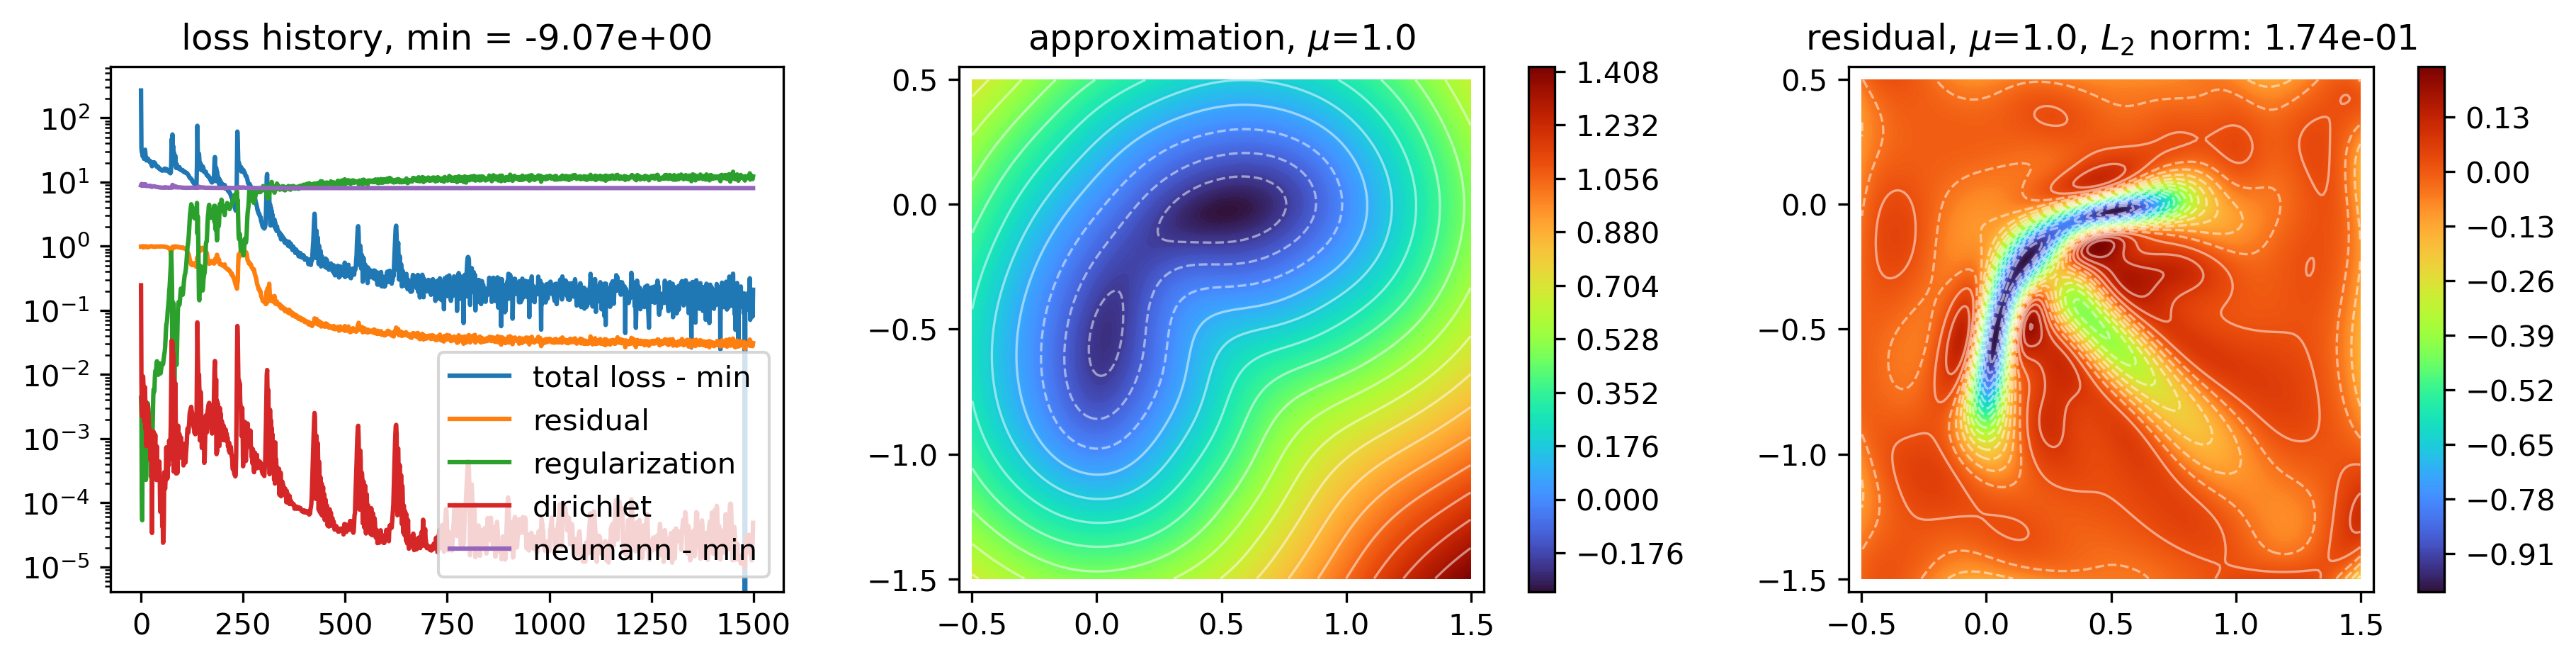
\includegraphics[width=\linewidth]{images/newlines/levelset/EikonalBean_curvature.png}

        % \vspace{10pt}

		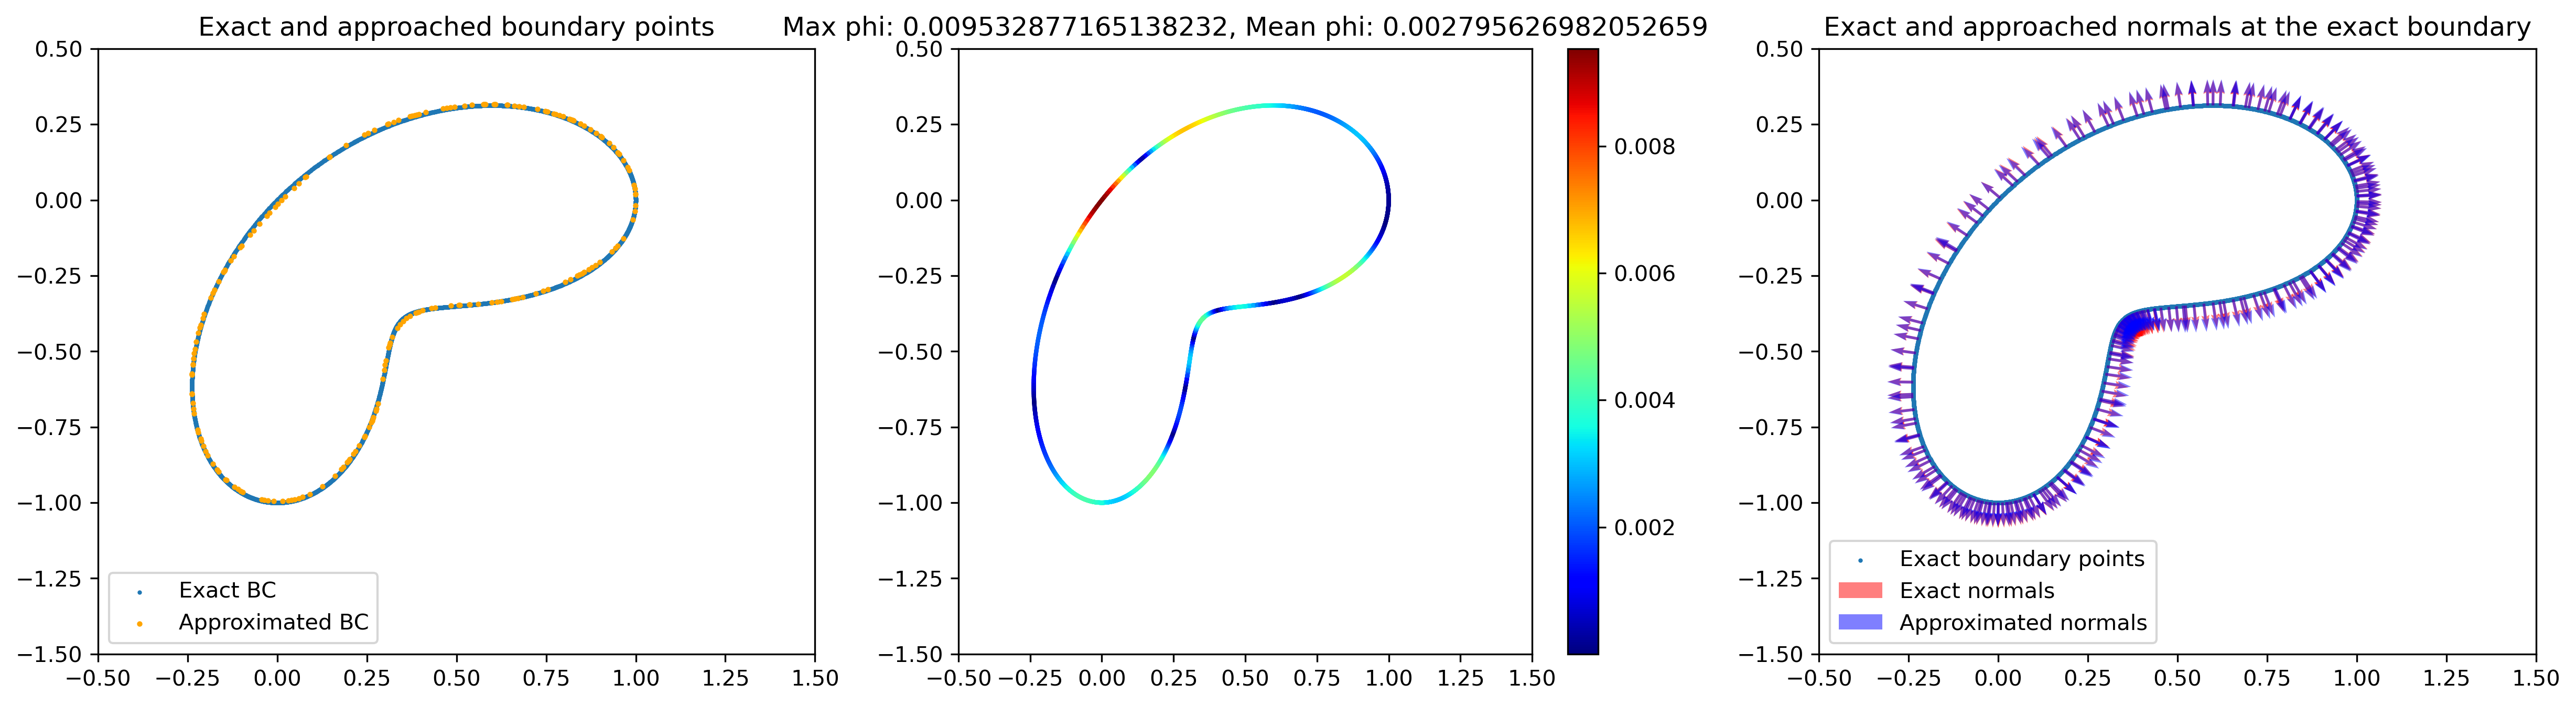
\includegraphics[width=\linewidth]{images/newlines/levelset/boundary_curvature.png}
	\end{figure}

    % \vspace{-5pt}
    % TODO : Ajouter résultats "Poisson on Bean" + Mettre au propre les images. 
\end{frame}

\subsection{\filledstar A posteriori error estimates}

\begin{frame}{Problem considered} 
	\textbf{Problem statement:} Considering the \textcolor{red}{Poisson problem with Dirichlet BC}:
	\vspace{-5pt}
	\begin{equation*}
		\left\{
		\begin{aligned}
			-\Delta u & = f, \; &  & \text{in } \; \Omega \times \mathcal{M}, \\
			u         & = 0, \;  &  & \text{on } \; \Gamma \times \mathcal{M},
		\end{aligned}
		\right.
		% \label{eq:Lap2DMixed}\tag{$\mathcal{P}$}
	\end{equation*}

	with $\Omega=[-0.5\pi,0.5\pi]^2$ and $\mathcal{M}=[-0.5,0.5]^2$ ($p=2$).
	
	\vspace{2pt}
	\textbf{Analytical solution :}

	\vspace{-12pt}
	\begin{equation*}
		% \label{eq:analytical_solution_Lap2D}
		u(\bm{x};\bm{\mu})= \exp\left(-\frac{(x-\mu_1)^2+(y-\mu_2)^2}{2(0.15)^2}\right)\sin(2x)\sin(2y).
	\end{equation*}

	\vspace{2pt}
	\small
	\textbf{PINN training:} Imposing Dirichlet BC exactly in the PINN.

	\vspace{8pt}
\end{frame}

\begin{frame}{Adaptive mesh refinement}	
    \textbf{Adaptive refinement loop} using Dorfler marking strategy. \refappendix{frame:amr} %(residual estimator)
    
    \begin{center}
        \textbf{Standard FEM}
        \vspace{2pt}

        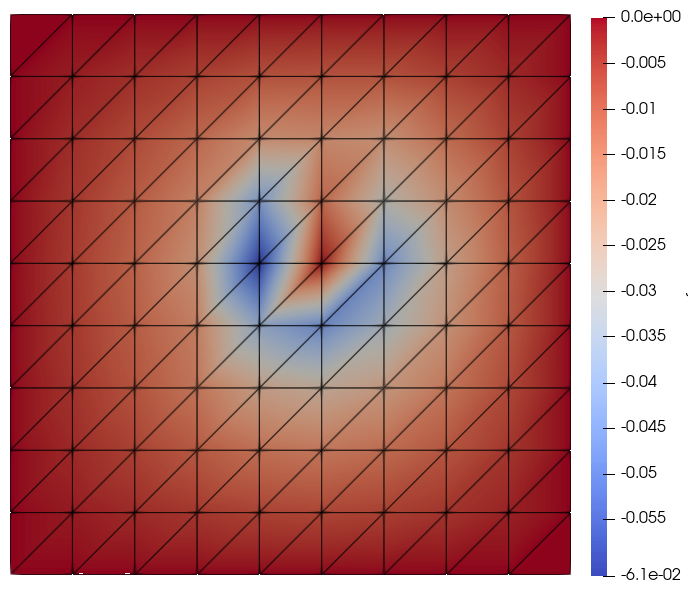
\includegraphics[width=0.2\linewidth]{images/newlines/mesh/explications/fem/u_h.png}
        \quad
        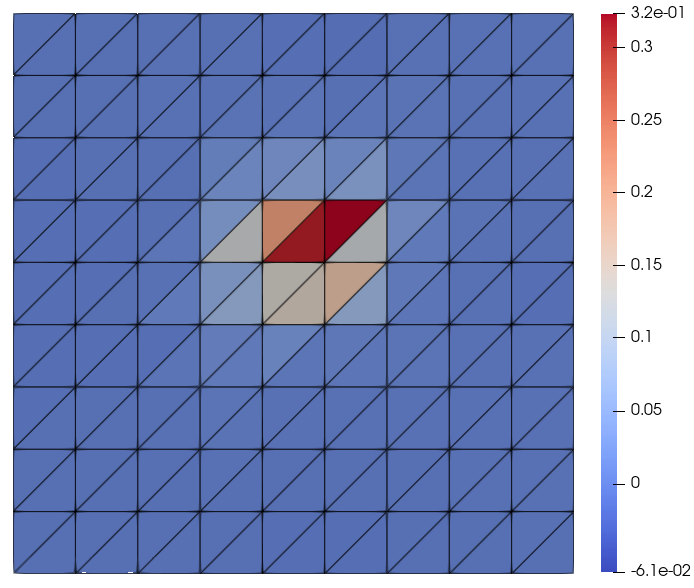
\includegraphics[width=0.2\linewidth]{images/newlines/mesh/explications/fem/eta_h.png}
        \quad
        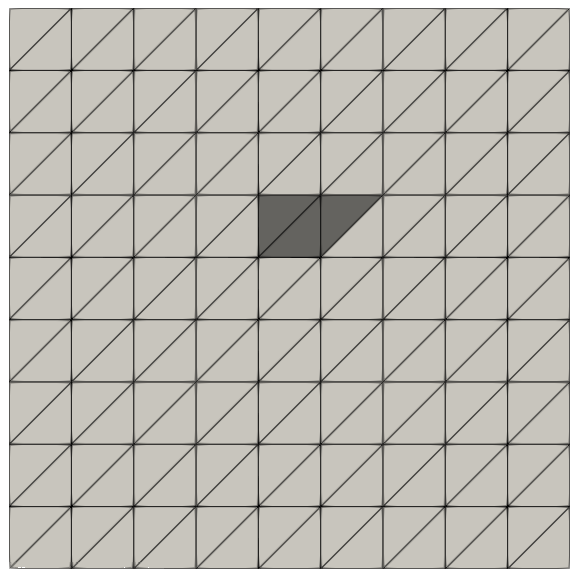
\includegraphics[width=0.17\linewidth]{images/newlines/mesh/explications/fem/marking.png}
        \qquad
        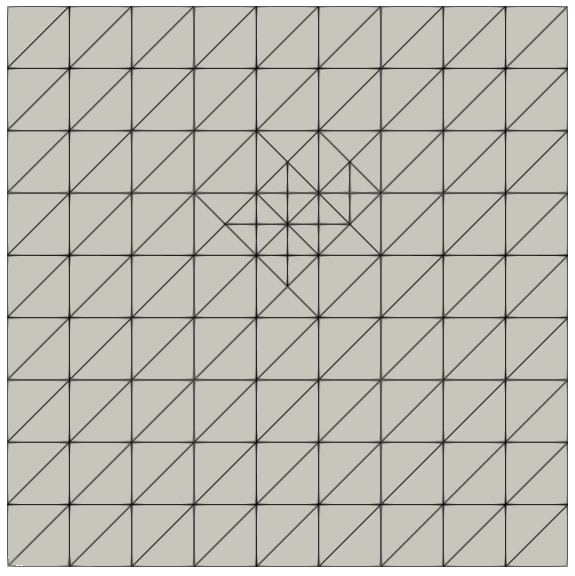
\includegraphics[width=0.17\linewidth]{images/newlines/mesh/explications/fem/refined.png}
    \end{center}

    \vspace{-10pt}
    $\cdots\hspace{1pt}\longrightarrow\hspace{8pt}
    \text{SOLVE}\hspace{18pt}\longrightarrow\hspace{6pt}
    \text{ESTIMATE}\hspace{8pt}\longrightarrow\hspace{14pt}
    \text{MARK}\hspace{14pt}\longrightarrow\hspace{8pt}
    \text{REFINE}\hspace{4pt}\longrightarrow\hspace{1pt}
    \cdots$

    \hspace{45pt}$\text{on }u_h\hspace{55pt}\eta_{res,T}$

    \vspace{8pt}
    \textbf{Local residual estimator (in $L^2$ norm):} Let $T$ be a cell of $\mathcal{T}_h$ .

    \vspace{-8pt}
    % $$\eta_{res,T}^2 = h_T^4 \|\Delta u_h + f_h\|_{L^2(T)}^2 + \frac{1}{2} \sum_{E \in \partial T} h_E^2 \|[\nabla u_h\cdot n]\|_{L^2(E)}^2$$
    $$\eta_{res,T}^2 = h_T^2 \|\Delta u_h + f_h\|_{L^2(T)}^2 + \frac{1}{2} \sum_{E \in \partial T} h_E \|[\nabla u_h\cdot n]\|_{L^2(E)}^2$$
    with $h_\bullet$ the size of $\bullet$ and considering the Poisson problem.

    % Considering the Poisson problem with Dirichlet boundary conditions.

    % (en précisant que c'est le coût du solve qui est le plus important)
\end{frame}

\begin{frame}[noframenumbering]{Adaptive mesh refinement}	
    \textbf{Adaptive refinement loop} using Dorfler marking strategy.
    
    \begin{center}
        \textcolor{red}{\textbf{Additive Approach}}
        \vspace{2pt}

        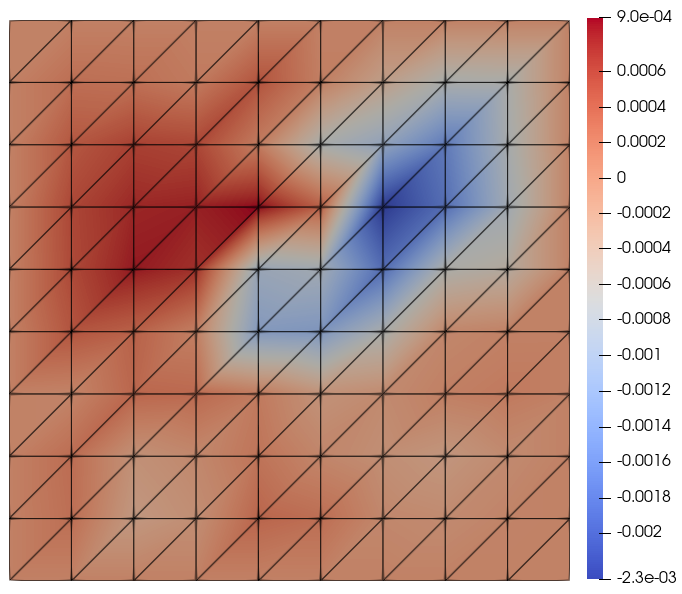
\includegraphics[width=0.2\linewidth]{images/newlines/mesh/explications/add/p_h.png}
        \quad
        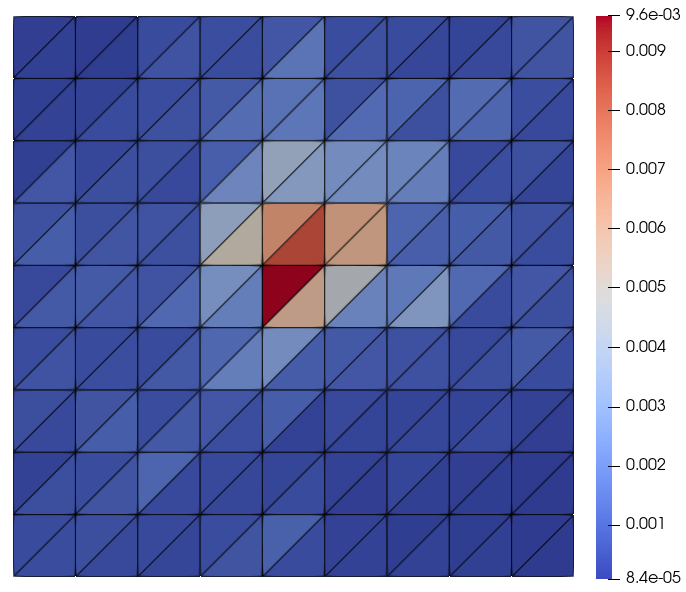
\includegraphics[width=0.2\linewidth]{images/newlines/mesh/explications/add/eta_h_add.png}
        \quad
        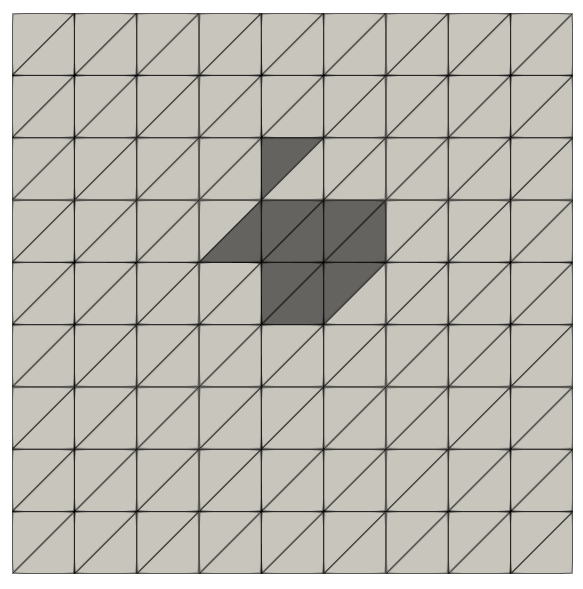
\includegraphics[width=0.17\linewidth]{images/newlines/mesh/explications/add/marking_add.png}
        \qquad
        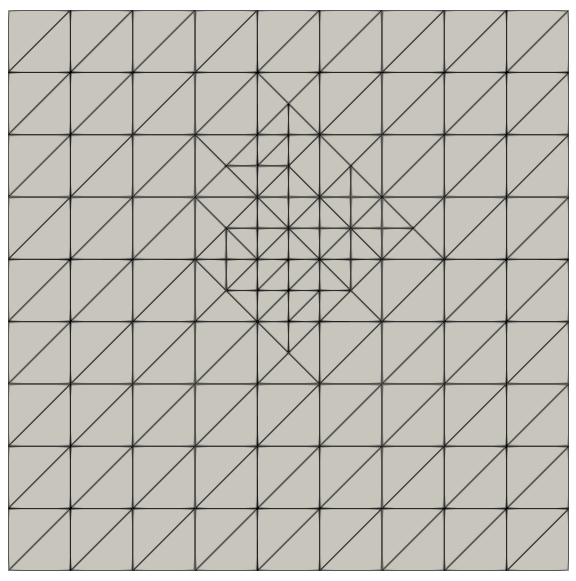
\includegraphics[width=0.17\linewidth]{images/newlines/mesh/explications/add/refined_add.png}
    \end{center}

    \vspace{-10pt}
    $\cdots\hspace{1pt}\longrightarrow\hspace{8pt}
    \text{SOLVE}\hspace{18pt}\longrightarrow\hspace{6pt}
    \text{ESTIMATE}\hspace{8pt}\longrightarrow\hspace{14pt}
    \text{MARK}\hspace{14pt}\longrightarrow\hspace{8pt}
    \text{REFINE}\hspace{4pt}\longrightarrow\hspace{1pt}
    \cdots$

    \hspace{45pt}$\text{on }\textcolor{red}{p_h^+}\hspace{55pt}\eta_{res,T}$

    \vspace{8pt}
    \textbf{Local residual estimator (in $L^2$ norm):} Let $T$ be a cell of $\mathcal{T}_h$ .

    \vspace{-8pt}
    % $$\eta_{res,T}^2 = h_T^4 \|\textcolor{red}{\big((\Delta u_\theta)_h + \Delta p_h^+\big) + f_h}\|_{L^2(T)}^2 + \frac{1}{2} \sum_{E \in \partial T} h_E^2 \|\textcolor{red}{[\nabla p_h^+\cdot n]}\|_{L^2(E)}^2$$
    $$\eta_{res,T}^2 = h_T^2 \|\textcolor{red}{\big((\Delta u_\theta)_h + \Delta p_h^+\big) + f_h}\|_{L^2(T)}^2 + \frac{1}{2} \sum_{E \in \partial T} h_E \|\textcolor{red}{[\nabla p_h^+\cdot n]}\|_{L^2(E)}^2$$
    with $h_\bullet$ the size of $\bullet$ and considering the Poisson problem.
\end{frame}

\begin{frame}[noframenumbering]{Adaptive mesh refinement}	
    \textbf{Adaptive refinement loop} using Dorfler marking strategy.
    
    \begin{center}
        \textbf{Additive Approach \textcolor{red}{- No resolution}}
        \vspace{2pt}

        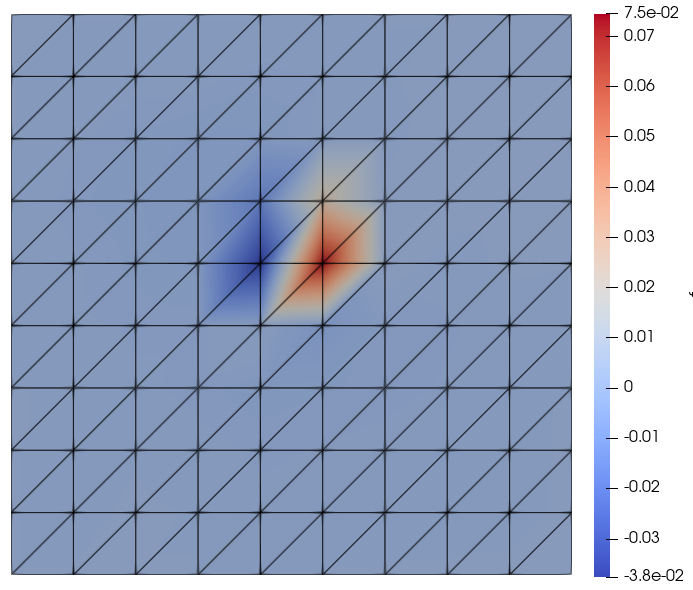
\includegraphics[width=0.2\linewidth]{images/newlines/mesh/explications/addnet/u_theta_h.png}
        \quad
        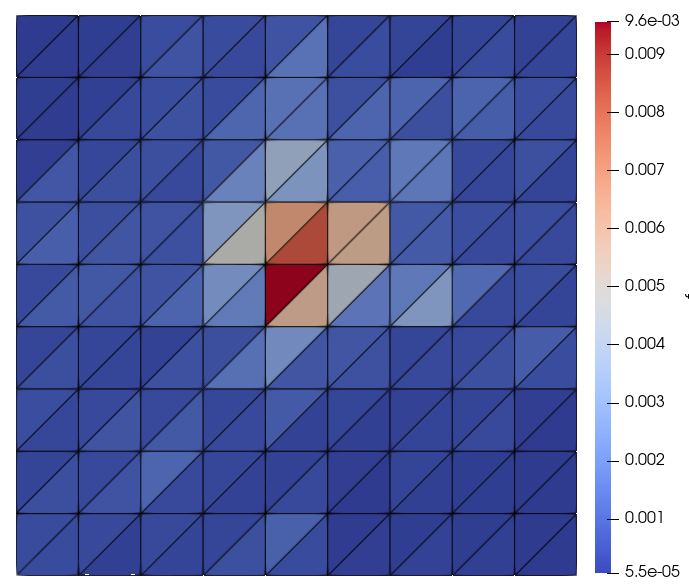
\includegraphics[width=0.2\linewidth]{images/newlines/mesh/explications/addnet/eta_h_addnet.png}
        \quad
        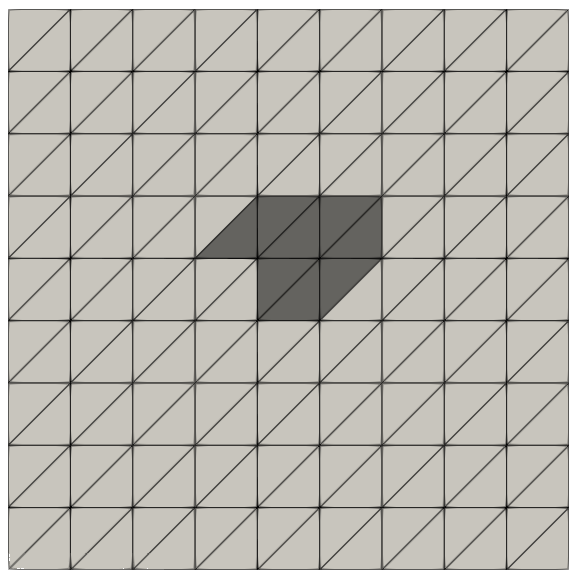
\includegraphics[width=0.17\linewidth]{images/newlines/mesh/explications/addnet/marking_addnet.png}
        \qquad
        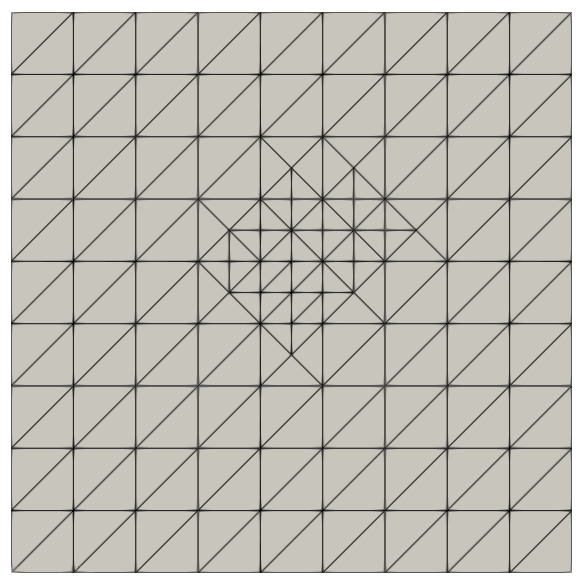
\includegraphics[width=0.17\linewidth]{images/newlines/mesh/explications/addnet/refined_addnet.png}
    \end{center}

    \vspace{-10pt}
    $\cdots\longrightarrow
    \textcolor{red}{\text{INTERPOLATE}}\longrightarrow\hspace{6pt}
    \text{ESTIMATE}\hspace{8pt}\longrightarrow\hspace{14pt}
    \text{MARK}\hspace{14pt}\longrightarrow\hspace{8pt}
    \text{REFINE}\hspace{4pt}\longrightarrow\hspace{1pt}
    \cdots$

    \hspace{55pt}$\textcolor{red}{u_\theta}\hspace{55pt}\eta_{res,T}$

    \vspace{8pt}
    \textbf{Local residual estimator (in $L^2$ norm):} Let $T$ be a cell of $\mathcal{T}_h$ .

    \vspace{-8pt}
    % $$\eta_{res,T}^2 = h_T^4 \|\textcolor{red}{(\Delta u_\theta)_h + f_h}\|_{L^2(T)}^2$$
    $$\eta_{res,T}^2 = h_T^2 \|\textcolor{red}{(\Delta u_\theta)_h + f_h}\|_{L^2(T)}^2$$
    with $h_\bullet$ the size of $\bullet$ and considering the Poisson problem.
\end{frame}

\begin{frame}{Numerical results}
    \vspace{-10pt}
    \begin{center}
        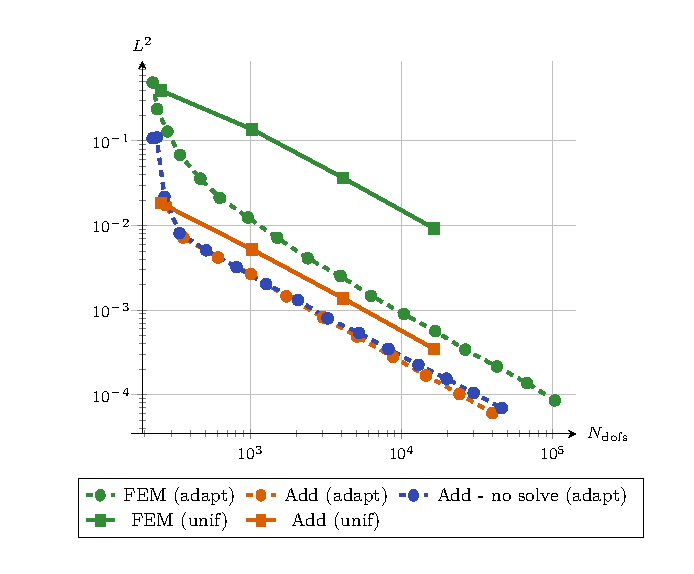
\includegraphics[width=0.4\linewidth]{images/newlines/mesh/results/cvg.pdf}
        \includegraphics[width=0.4\linewidth]{images/newlines/mesh/results/times.pdf}
    \end{center}
    
    \vspace{-10pt}
    \footnotesize
    \warning \quad Results obtained on a laptop GPU (Time measurements polluted by external factors).
    
    \normalsize
    \vspace{5pt}
    \textbf{Ideas for improving results :} Additive approach (no resolution).

    \vspace{3pt}
    \begin{minipage}{0.1\linewidth}
        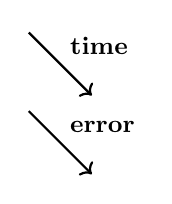
\begin{tikzpicture}[scale=1]
            \draw[->, thick] (0,1.8) -- (0.8,1);
            \node[above right] at (0.4,1.4) {\textbf{time}};

            \draw[->, thick] (0,0.8) -- (0.8,0);
            \node[above right] at (0.4,0.4) {\textbf{error}};
        \end{tikzpicture}
    \end{minipage} \hspace{5pt}
    \begin{minipage}{0.86\linewidth}
        \vspace{2pt}
        Interpolate only mesh points added in the refinement process. \\

        \vspace{5pt}
        Use another metric such as curvature, rather than residual error.

        % \vspace{-5pt}
        % $$\Delta u_\theta+f \qquad \ne \qquad u-u_\theta$$
    \end{minipage}
    % \begin{itemize}
    %     \item To improve execution times: \\ 
    %     Interpolate only mesh points added in the refinement process.
    %     % \item Cout du passage sur GPU.
    %     \item To improve the mesh : \\
    %     Use another metric such as curvature, rather than residual error. \\
    %     (The network residual ($\Delta u_\theta+f$) does not match the additive solution (the network error $u-u_\theta$).)

    % \end{itemize}

\end{frame}

\subsection{\filledstar Non linear PDEs}

\begin{frame}{Problem considered}	
    \textbf{Objective:} Extend the additive approach to non linear PDEs.

    \vspace{10pt}
    \textbf{Problem statement:} Considering the \textcolor{red}{non linear Poisson problem with Dirichlet BC}:
    \vspace{-5pt}
    \begin{equation*}
        \left\{
        \begin{aligned}
            -\text{div}\big((1+4u^4)\nabla u\big) & = f, \; &  & \text{in } \; \Omega, \\
            u         & = 1, \;  &  & \text{on } \; \partial\Omega.
        \end{aligned}
        \right.
    \end{equation*}

    with $\Omega=[-0.5\pi,0.5\pi]^2$ and $\mathcal{M}=[-0.5,0.5]^2$ ($p=2$).

    \vspace{5pt}
	\textbf{Analytical solution :}

	\vspace{-12pt}
	\begin{equation*}
		u(\bm{x};\bm{\mu})= 1 + \exp\left(-\frac{(x-\mu_1)^2+(y-\mu_2)^2}{2}\right)\sin(2x)\sin(2y)
	\end{equation*}
	\vspace{-5pt}
	
    \vspace{5pt}
	\textbf{PINN training:} Imposing BC exactly with a level-set function.

\end{frame}

\begin{frame}{Newton method}
    

    We want to solve the non linear system: \hfill \tiny $N_h$ : number of degrees of freedom.

    \normalsize
    \vspace{-10pt}
    \begin{equation}
        \label{eq:nonlinear}
        F(u) = 0 
    \end{equation}

    \vspace{-2pt}
    with $F:\mathbb{R}^{N_h} \to \mathbb{R}^{N_h}$ a non linear operator and $u\in\mathbb{R}^{N_h}$ the unknown vector.

    \begin{center}
        \small
        \begin{minipage}{0.9\linewidth}
            \begin{algorithm}[H]
                \SetAlgoLined
                \caption{Newton's method to solve \eqref{eq:nonlinear} \citep{newton_accel_2025}}
                \textbf{Initialization step:} set $u^{(0)} = u_0$\;
                \For{\( k \ge 0 \)}{
                    Solve the linear system \( F(u^{(k)}) + F'(u^{(k)}) \delta^{(k+1)} = 0 \) for \( \delta^{(k+1)} \)\;
                    Update \( u^{(k+1)} = u^{(k)} + \delta^{(k+1)} \)\;
                }
            \end{algorithm}
        \end{minipage}
    \end{center}

    \vspace{5pt}
    \textbf{Standard version:} \\
    Initialization with a constant value $u_0$. For instance, $u_0=1$.

    \vspace{5pt}
    \textbf{DeepPhysics version:} \citep{odot_deepphysics_2021} \\
    Initialization with a PINN solution $u_0=u_\theta$.
\end{frame}

\begin{frame}[noframenumbering]{Newton method}
    \vspace{5pt}
    We want to solve the non linear system: \hfill \tiny $N_h$ : number of degrees of freedom.

    \normalsize
    \vspace{-10pt}
    \begin{equation}
        F(\textcolor{red}{p_+ + u_\theta}) = 0 \tag{1}
    \end{equation}

    \vspace{-2pt}
    with $F:\mathbb{R}^{N_h} \to \mathbb{R}^{N_h}$ a non linear operator and $\textcolor{red}{p_+}\in\mathbb{R}^{N_h}$ the unknown vector.

    \begin{center}
        \small
        \begin{minipage}{0.9\linewidth}
            \begin{algorithm}[H]
                \SetAlgoLined
                \caption{\textcolor{red}{Additive approach} to solve \eqref{eq:nonlinear} }
                \textbf{Initialization step:} set \textcolor{red}{$p_+^{(0)} = 0$}\;
                \For{\( k \ge 0 \)}{
                    Solve the linear system \( F(\textcolor{red}{p_+^{(k)}+u_\theta}) + F'(\textcolor{red}{p_+^{(k)}+u_\theta}) \delta^{(k+1)} = 0 \) for \( \delta^{(k+1)} \)\;
                    Update \( \textcolor{red}{p_+^{(k+1)}} = \textcolor{red}{p_+^{(k)}} + \delta^{(k+1)} \)\;
                }
            \end{algorithm}
        \end{minipage}
    \end{center}

    \textbf{Advantage compared to DeepPhysics:}

    \begin{center}
    $u_\theta$ is not required to live in the same space as $p_+$.
    \end{center}
\end{frame}

\begin{frame}{Numerical results}	
    \vspace{-10pt}
    \begin{center}
        \begin{minipage}{0.54\linewidth}
            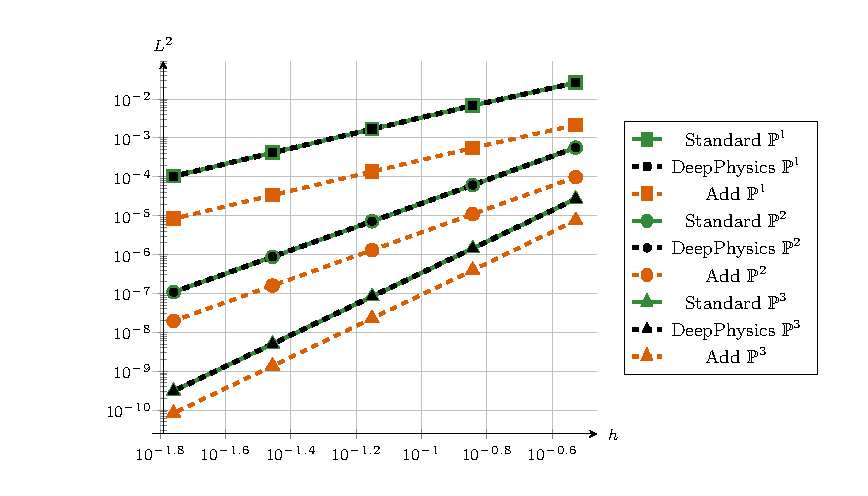
\includegraphics[width=\linewidth]{images/newlines/nonlinear/results/cvg_cropped.pdf}
        \end{minipage}
        \begin{minipage}{0.42\linewidth}
            \small
            \textbf{Number of iterations :}

            \begin{itemize}
                \item Standard Newton: $8$ iterations.
                \item DeepPhysics: $4$ iterations.
                \item Additive approach: $4$ iterations.
            \end{itemize}
        \end{minipage}
        
        \vspace{-6pt}
        \includegraphics[width=\linewidth]{images/newlines/nonlinear/results/times.pdf}
    \end{center}
\end{frame}

	\renewcommand{\insertsectionheadSubtitle}{
		\begin{itemize}
			\item Results obtained with a laptop GPU.
			\item The newton solver is the same for all methods (rtol$=10^{-10}$, atol$=10^{-10}$, max\_it$=30$).
			\item Additive approach : we consider $u_\theta$ in a $\mathbb{P}_3^2\times \mathbb{P}_2 \times \mathbb{P}_3$ continuous Lagrange FE space (defined on the current mesh).
		\end{itemize}}
	\section{Numerical results}
	\documentclass[french]{article}
\usepackage[T1]{fontenc}
\usepackage[utf8]{inputenc}
\usepackage[french]{babel}
\usepackage{amsmath}
\usepackage{mathtools}
\usepackage{color}
\usepackage[svgnames,dvipsnames]{xcolor} 
\usepackage{soul}
\usepackage{amssymb}
\usepackage{enumitem}
\usepackage{multicol}
\usepackage[left=2cm,right=2cm,top=2cm,bottom=2cm]{geometry}
\newcommand{\mathcolorbox}[2]{\colorbox{#1}{$\displaystyle #2$}}
\usepackage{pifont}
\usepackage{pst-all}
\usepackage{pstricks}
\usepackage{delarray}
\usepackage{setspace}
\usepackage{graphicx}
\usepackage{hyperref}
\usepackage{nicematrix}
\usepackage{listings}
\usepackage{float}

\hypersetup{
	colorlinks=true,
	linkcolor=blue,
	filecolor=magenta,      
	urlcolor=cyan,
	pdfpagemode=FullScreen,
}

\usepackage{amsthm}
\newtheorem*{Rem}{Remarque}

\newenvironment{conclusion}[1]{%
	\begin{center}\normalfont\textbf{Conclusion}\end{center}
	\begin{quotation} #1 \end{quotation}
}{%
	\vspace{1cm}
}

\newcommand\pythonstyle{\lstset{
	language=Python,
	basicstyle=\ttm,
	morekeywords={self},              % Add keywords here
	keywordstyle=\ttb\color{deepblue},
	emph={MyClass,__init__},          % Custom highlighting
	emphstyle=\ttb\color{deepred},    % Custom highlighting style
	stringstyle=\color{deepgreen},
	frame=tb,                         % Any extra options here
	showstringspaces=false
}}

\lstdefinestyle{Cpp}{
	language=C++,
	tabsize=3,
	basicstyle=\ttfamily,
	keywordstyle=\color{blue}\ttfamily,
	stringstyle=\color{red}\ttfamily,
	commentstyle=\color{green}\ttfamily,
	morecomment=[l][\color{magenta}]{\#}
}

\lstdefinestyle{Python}{
	language=Python,
	tabsize=3,
	basicstyle=\ttfamily,
	keywordstyle=\color{blue}\ttfamily,
	stringstyle=\color{red}\ttfamily,
	commentstyle=\color{green}\ttfamily,
	morecomment=[l][\color{magenta}]{\#}
}

\lstset{style=Cpp}

\setlength\parindent{0pt}
\usepackage[skip=2pt]{caption}

\usepackage{fontawesome}

\usepackage{lipsum}

\begin{document}
	LECOURTIER Frédérique \hfill \today
	\begin{center}
		\Large\textbf{{Results : Week 1 - Week 7}}
	\end{center}
	\tableofcontents
	\newpage

	\section{Week 4 : 23/10/2023 - 27/10/2023}
	\graphicspath{{weeks/images/week_4/}}

\subsection{Reproduction résultats - Article 2104.08426}

Dans un premier temps, j'ai cherché à implémenter en Python les deux méthodes présentées dans l'article 2104.08426, permettant de calculer une ADF ("Approach Distance Function"). On retrouve le calcul d'une ADF sur un polygone qui représente le bord d'une ellipse par les deux méthodes suivantes :  la méthode REQ (R-equivalence) dans la Figure \ref{REQ} et la méthode MVP ("Mean Value Potential") dans la Figure \ref{MVP}.

\begin{minipage}{0.38\linewidth}
	\begin{figure}[H]
		\centering
		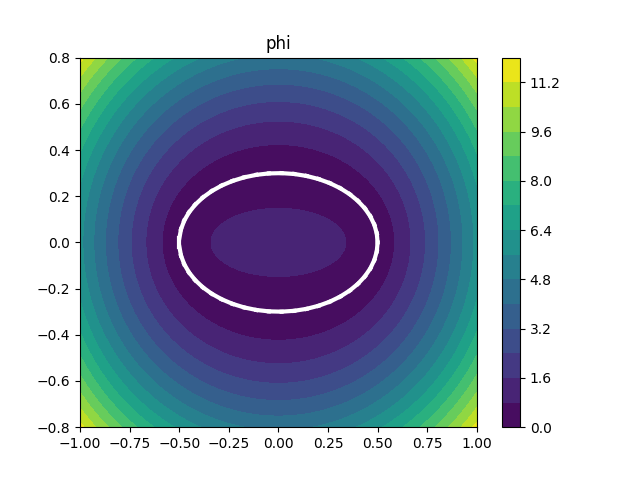
\includegraphics[width=0.7\linewidth]{"article/REQ_ellipse.png"}
		\caption{ADF par REQ sur une ellipse.}
		\label{REQ}
	\end{figure}
\end{minipage}
\begin{minipage}{0.58\linewidth}
	\begin{figure}[H]
		\centering
		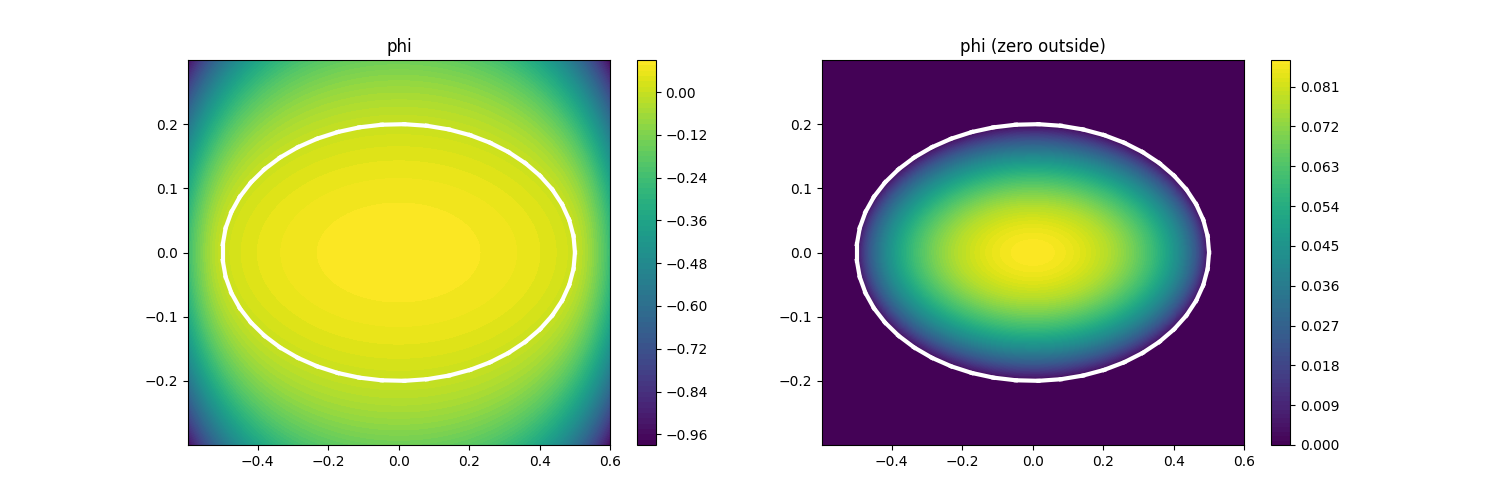
\includegraphics[width=\linewidth]{"article/MVP_ellipse.png"}
		\caption{ADF par MVP sur une ellipse.}
		\label{MVP}
	\end{figure}
\end{minipage}

\subsection{Entraînement du PINNs à apprendre une solution unique}

\subsubsection{Problème considéré}

\textbf{EDP :} On considère le problème de Poisson avec condition de Dirichlet homogène ($g=0$), définie par

Trouver $u : \Omega \rightarrow \mathbb{R}^d (d=1,2,3)$ tel que
\begin{equation}
	\left\{
	\begin{aligned}
		-\Delta u &= f, \; &&\text{dans } \; \Omega, \\
		u&=g, \; &&\text{sur } \; \partial\Omega,
	\end{aligned}
	\right. \tag{$\mathcal{P}$} \label{pb_initial}
\end{equation}
avec $\Delta$ l'opérateur de Laplace.

\textbf{Géométrie :} On considère $\Omega$ comme étant un cercle de rayon $r$ et de centre $(x_0,y_0)$. 

Pour simplifier, on va considérer que $\Omega$ est entièrement contenu dans un carré $\mathcal{O}$ (Figure \ref{geom_circle}). 

\begin{minipage}{0.38\linewidth}
	\begin{figure}[H]
		\centering
		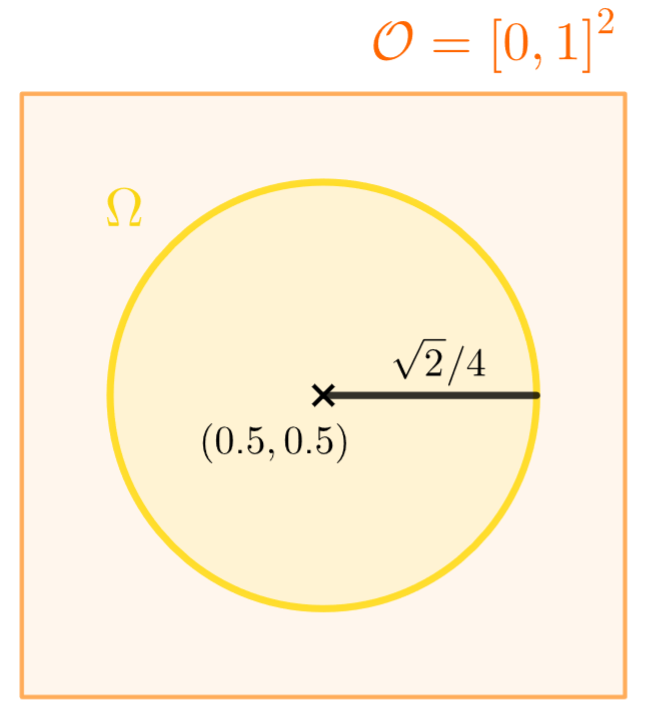
\includegraphics[width=0.7\linewidth]{"training/geom_circle.png"}
		\caption{Domaine considéré.}
		\label{geom_circle}
	\end{figure}
\end{minipage}
\begin{minipage}{0.68\linewidth}
	On considère la solution analytique $u_{ex}$, définie par
	\begin{equation*}
		u_{ex}(x,y)=S\times\sin\left(\frac{1}{r^2}\pi((x-x_0)^2+(y-y_0)^2)\right)
	\end{equation*}
	
	Ce qui nous fournit le terme source $f$, définie par
	\begin{align*}
		f(x,y)=\frac{4}{r^4}\pi^2&S((x-x_0)^2+(y-y_0)^2)\sin\left(\frac{1}{r^2}\pi((x-x_0)^2+(y-y_0)^2)\right) \\
		&-\frac{4}{r^2}\pi S \cos\left(\frac{1}{r^2}\pi((x-x_0)^2+(y-y_0)^2)\right)
	\end{align*}
\end{minipage}
\begin{Rem}
	On voit que sur le cercle, le problème est bien homogène.
	
	De plus, on notera qu'un choix simple peut être de prendre le carré $[x_0-r-\epsilon,x_0+r+\epsilon]\times[y_0-r-\epsilon,y_0+r+\epsilon]$ où $\epsilon>0$ est un paramètre fixé dans le but que $\Omega$ soit entièrement compris dans $\mathcal{O}$.
\end{Rem}

\subsubsection{Entraînement du PINNs}

On fixe $r=\sqrt{2}/4$, $(x_0,y_0)=(0.5,0.5)$ et $S=0.5$ et on considère ici que l'on souhaite entraîner un PINNs à apprendre cette solution. On utilisera l'implémentation développé dans le module ScimBA\footnote{\url{https://sciml.gitlabpages.inria.fr/scimba/}}. 

On notera que l'article 2104.08426 présente comment imposer les conditions au bord de manière exacte. C'est pourquoi, on considérera deux cas :
\begin{enumerate}[label=\textbullet]
	\item on apprend directement la solution $u$. La loss totale regroupe alors la loss sur le résidu et la loss sur le bord.
	\item on apprend $w$ tel que $u=\phi w$ avec $\phi$ notre fonction levelset. La loss ne contient alors que la loss sur le résidu. 
\end{enumerate}
Ainsi, une première étape a été de rajouter, dans l'implémentation de ScimBa, la possibilité de définir un domaine à partir d'une fonction levelset. Ainsi pour obtenir un sampling de points à l'intérieur de $\Omega$, il suffit de générer un échantillon de point sur le carré $\mathcal{O}$ et de ne garder que les points tels que $\phi(x,y)<0$. Pour générer un échantillon de point sur le bord du domaine $\Omega$, on a fait le choix pour l'instant de prendre les points tels que $|\phi(x,y)|<\epsilon$ avec $\epsilon=1e-5$ (Figure \ref{sampling_0}).

\begin{figure}[H]
	\centering
	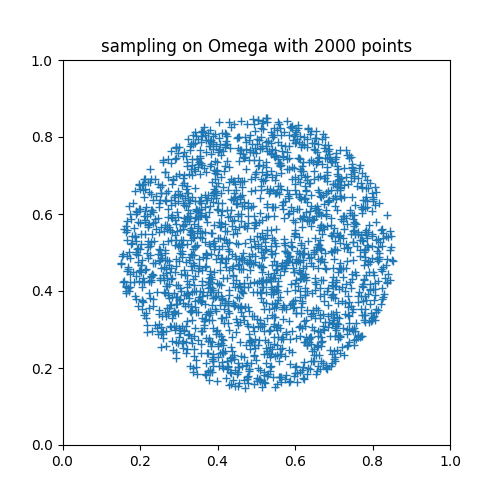
\includegraphics[width=0.5\linewidth]{"training/sampling_0.png"}
	\caption{Sampling à l'intérieur et au bord du cercle considéré.}
	\label{sampling_0}
\end{figure}

\begin{Rem}
	Pour le sampling du bord, c'est un choix qui ne sera pas conserver, il faudra trouver une solution plus rapide-précise que celle-ci.
\end{Rem}

On peut alors entraîner le PINNs à apprendre notre solution. On choisira la configuration suivante :
\begin{figure}[H]
	\centering
	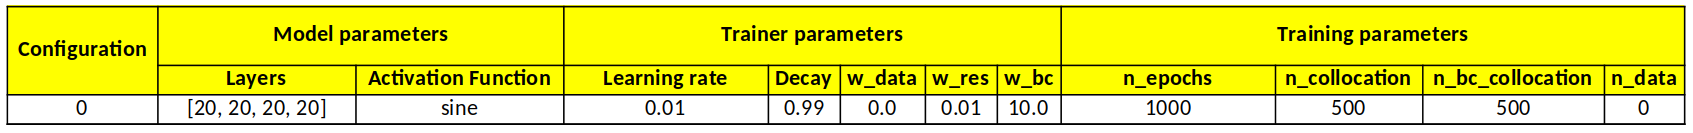
\includegraphics[width=\linewidth]{"training/config_0.png"}
	\caption{Paramètres d'entraînement considéré pour le PINNs.}
	\label{config_0}
\end{figure}

On va alors entraîner un modèle à apprendre $u$ (Figure \ref{model_0}) et un autre à apprendre $w$ (Figure \ref{model_0_exact_bc}) avec ces mêmes paramètres dans le but de comparer les résultats.

\begin{minipage}{0.48\linewidth}
	\begin{figure}[H]
		\centering
		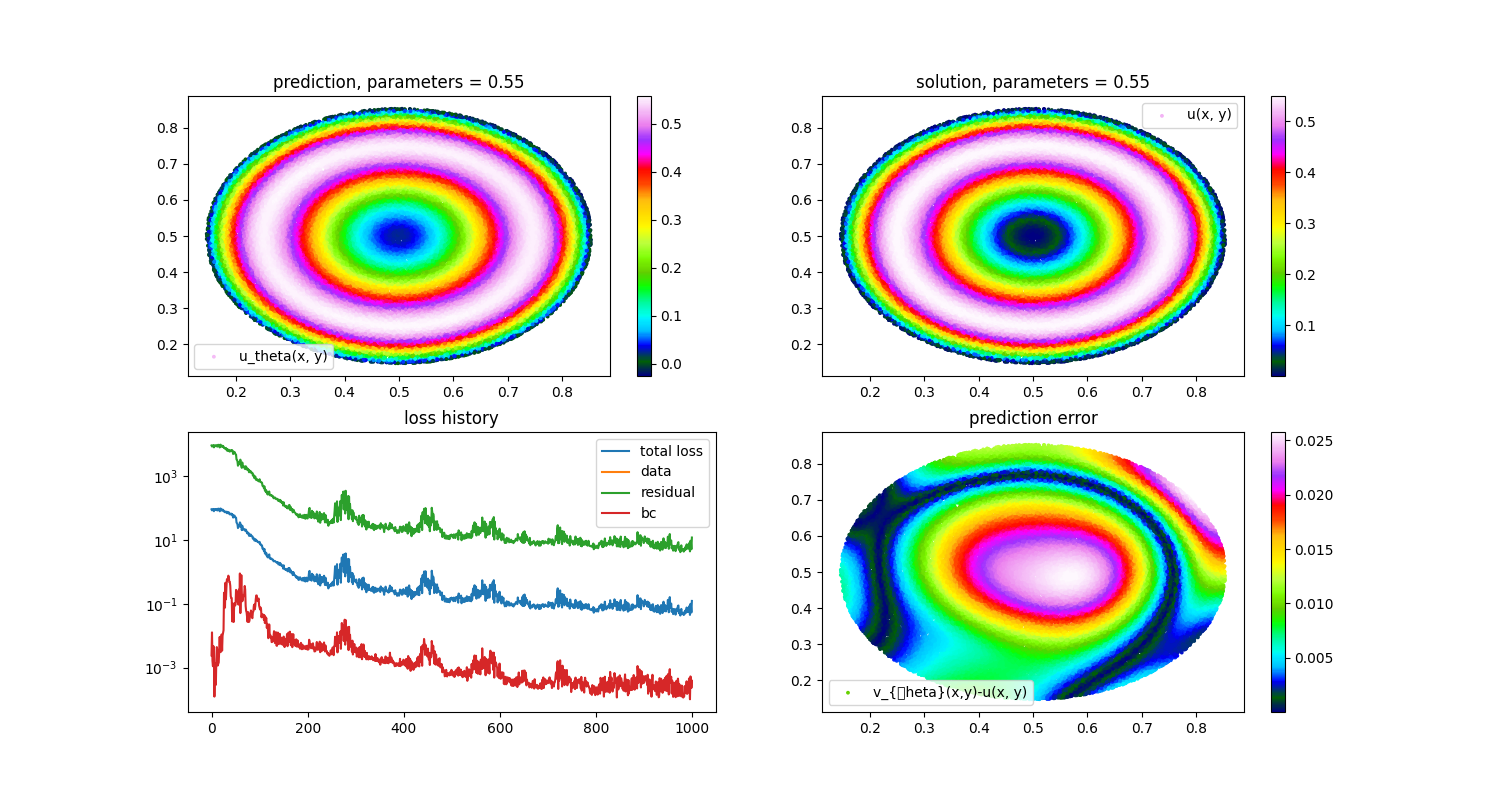
\includegraphics[width=\linewidth]{"training/model_0.png"}
		\caption{Fin d'entraînement - Modèle sur $u$.}
		\label{model_0}
	\end{figure}
\end{minipage}
\begin{minipage}{0.48\linewidth}
	\begin{figure}[H]
		\centering
		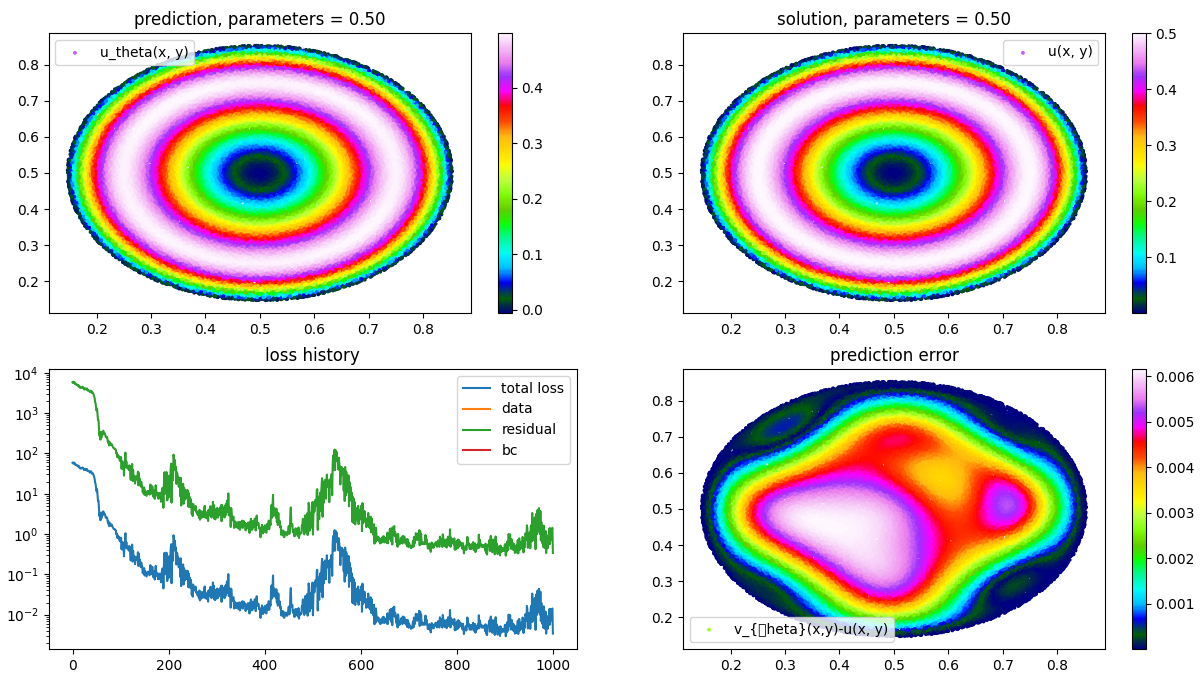
\includegraphics[width=\linewidth]{"training/model_0_exact_bc.png"}
		\caption{Fin d'entraînement - Modèle sur $w$.}
		\label{model_0_exact_bc}
	\end{figure}
\end{minipage}

\begin{Rem}
	Il semblerait que le modèle sur $w$ soit 10 fois plus précis en terme d'erreur.
	
	De plus, on remarque bien, sur la carte d'erreur, sur le modèle sur $u$ a des erreurs au bord, ce qui risque de poser problème dans la correction. 
\end{Rem}

\subsubsection{Correction sur les prédictions du PINNs}

On note $\tilde{\phi}$ la prédiction d'un des PINNs précédent. On ne va considérer ici que la correction par addition, on pose alors
\begin{equation*}
	\tilde{u}=\tilde{\phi}+\tilde{C}
\end{equation*}
et on cherche à trouver $\tilde{C}: \Omega \rightarrow \mathbb{R}^d$ solution du problème
\begin{equation*}
	\left\{\begin{aligned}
		-\Delta \tilde{u}&=f, \; &&\text{on } \Omega, \\
		\tilde{u}&=g, \; &&\text{in } \Gamma.
	\end{aligned}\right.
\end{equation*}
avec $g=0$ dans le cas considéré.
On cherche alors à trouver $\tilde{C}: \Omega \rightarrow \mathbb{R}^d$ solution du problème
\begin{equation*}
	\left\{\begin{aligned}
		-\Delta \tilde{C}&=\tilde{f}, \; &&\text{on } \Omega, \\
		\tilde{C}&=0, \; &&\text{in } \Gamma.
	\end{aligned}\right. %\tag{$\mathcal{C}_{+}$}
\end{equation*}
avec $\tilde{f}=f+\Delta\tilde{\phi}$.

On cherche alors à tester la correction sur les deux modèles précédents (celui où on apprend $u$ et celui où on apprend $w$). On testera l'utilisation de FEM et de $\phi$-FEM dans les deux cas.

\textbf{Résultats avec le modèle sur $u$ :}

\begin{minipage}{0.48\linewidth}
	\begin{figure}[H]
		\centering
		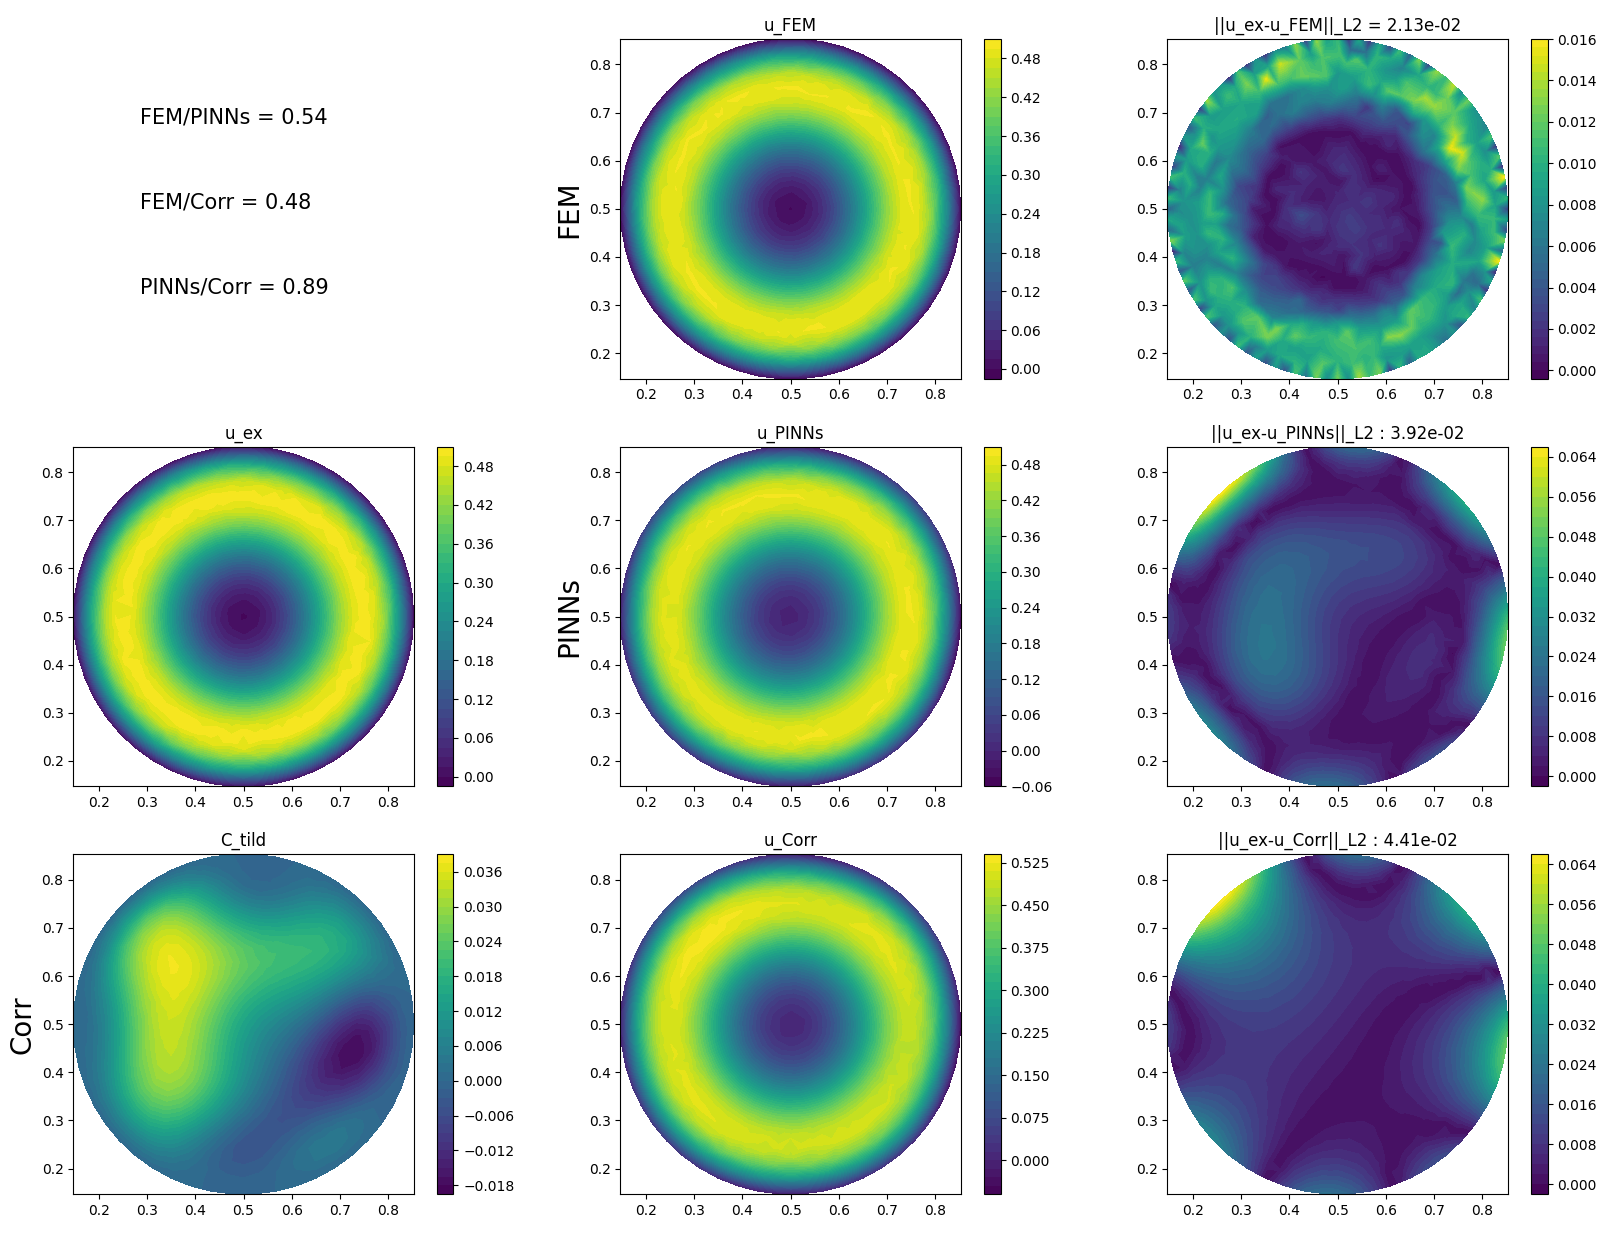
\includegraphics[width=\linewidth]{"corr/corr_fem_0.png"}
		\caption{Correction avec FEM - Modèle sur $u$.}
		\label{corr_fem_0}
	\end{figure}
\end{minipage}
\begin{minipage}{0.48\linewidth}
	\begin{figure}[H]
		\centering
		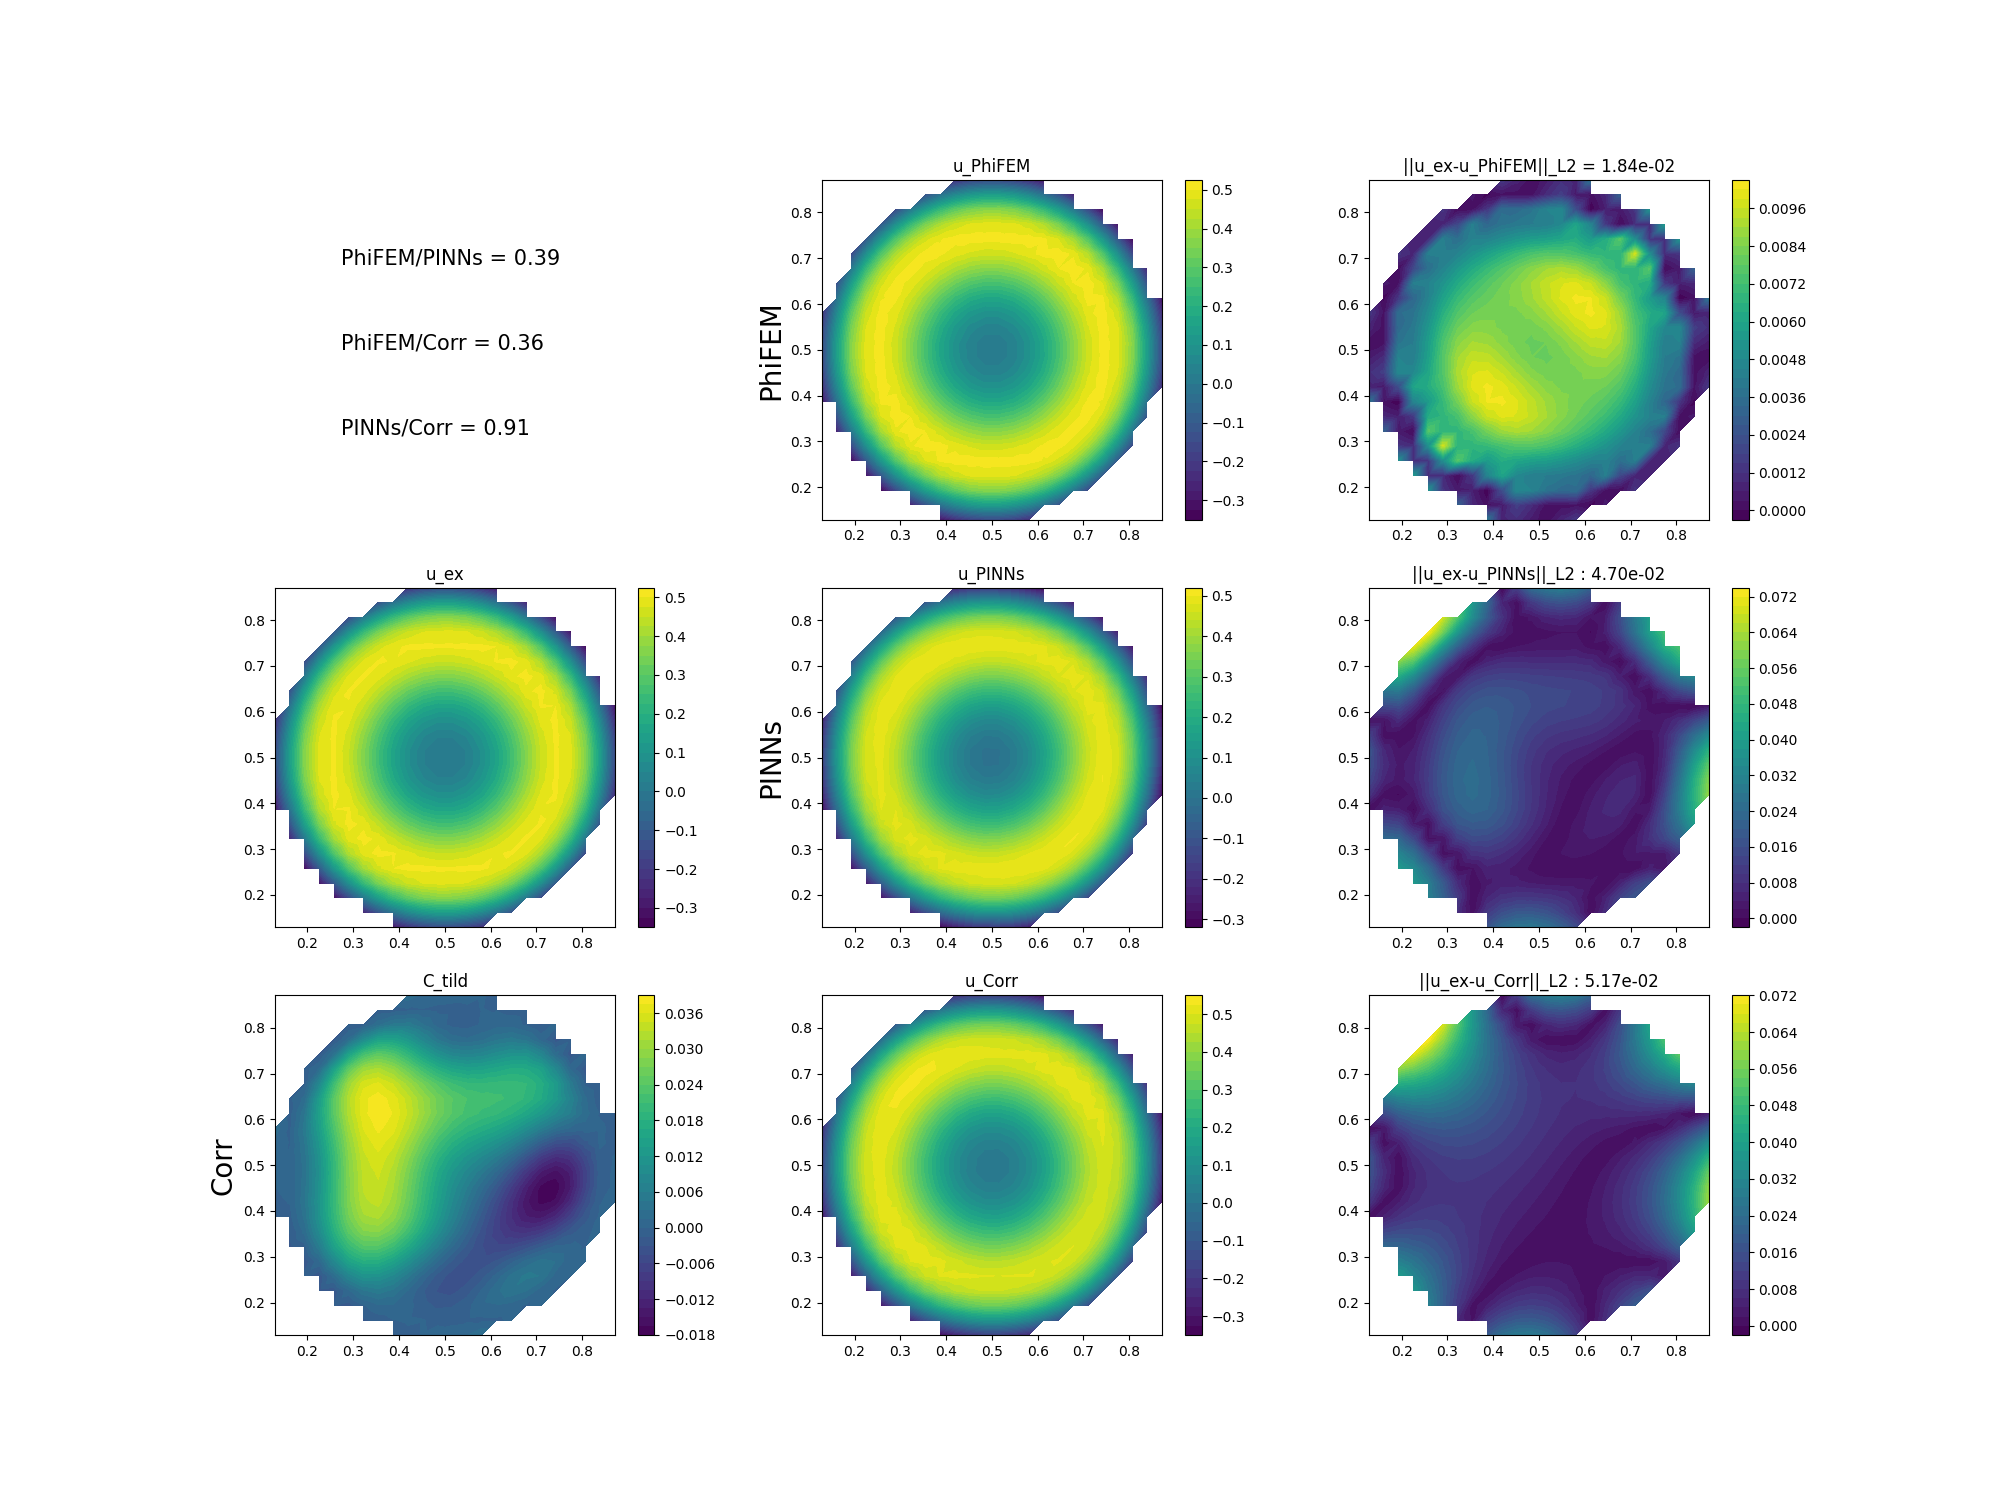
\includegraphics[width=\linewidth]{"corr/corr_phifem_0.png"}
		\caption{Correction avec $\phi$-FEM - Modèle sur $u$.}
		\label{corr_phifem_0}
	\end{figure}
\end{minipage}

\textbf{Résultats avec le modèle sur $w$ :}

\begin{minipage}{0.48\linewidth}
	\begin{figure}[H]
		\centering
		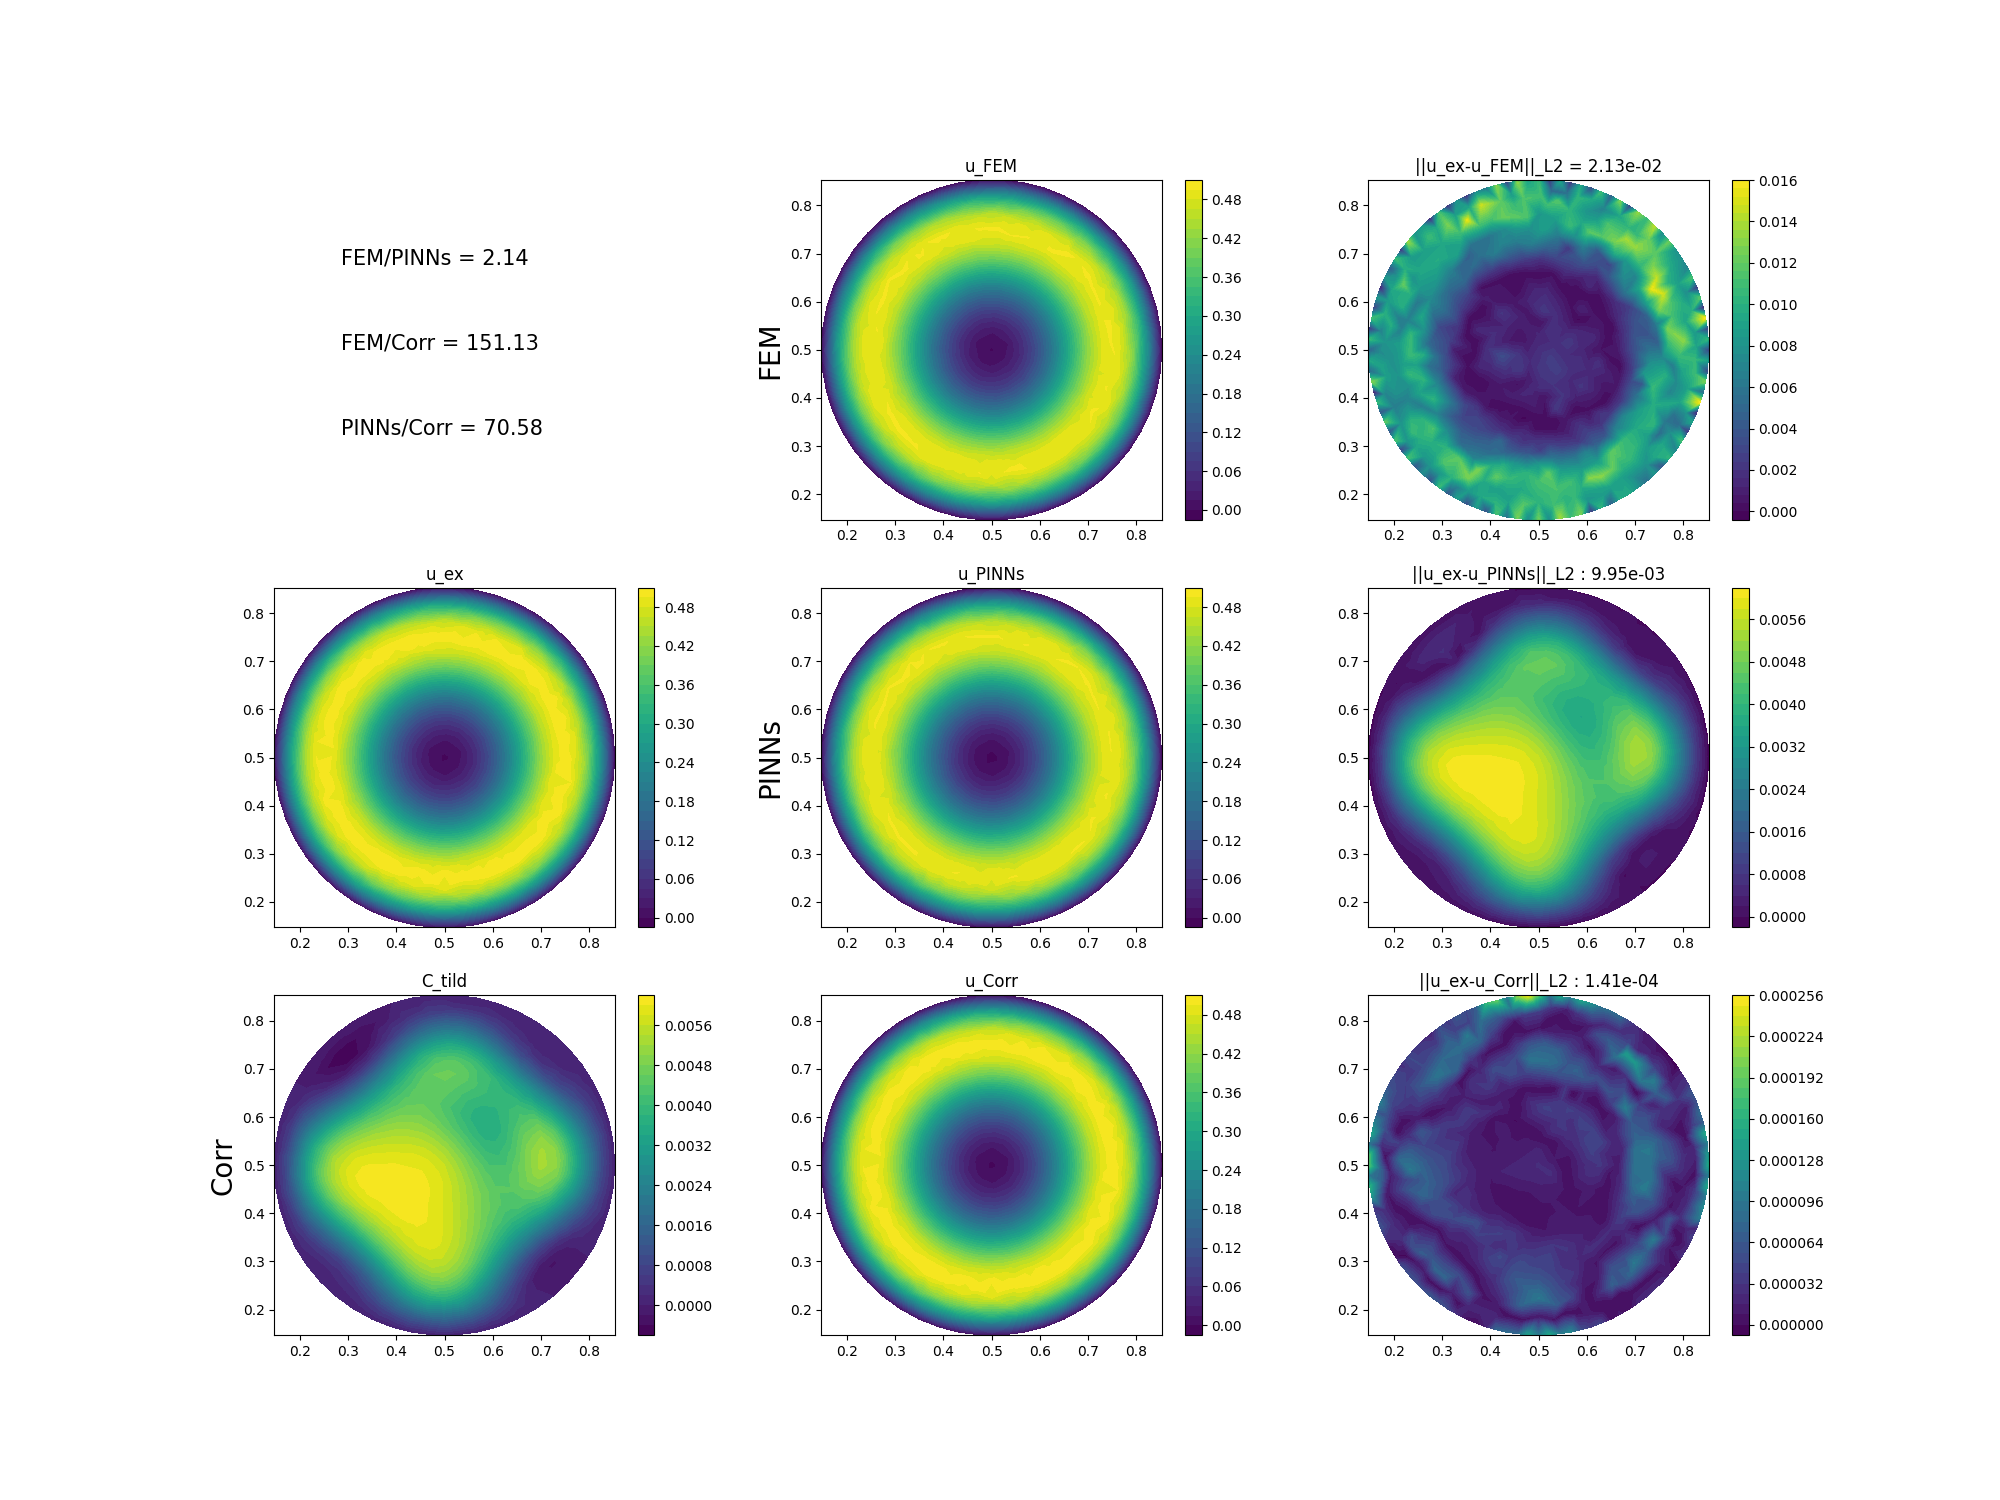
\includegraphics[width=\linewidth]{"corr/corr_fem_0_exact_bc.png"}
		\caption{Correction avec FEM - Modèle sur $w$.}
		\label{corr_fem_0_exact_bc}
	\end{figure}
\end{minipage}
\begin{minipage}{0.48\linewidth}
	\begin{figure}[H]
		\centering
		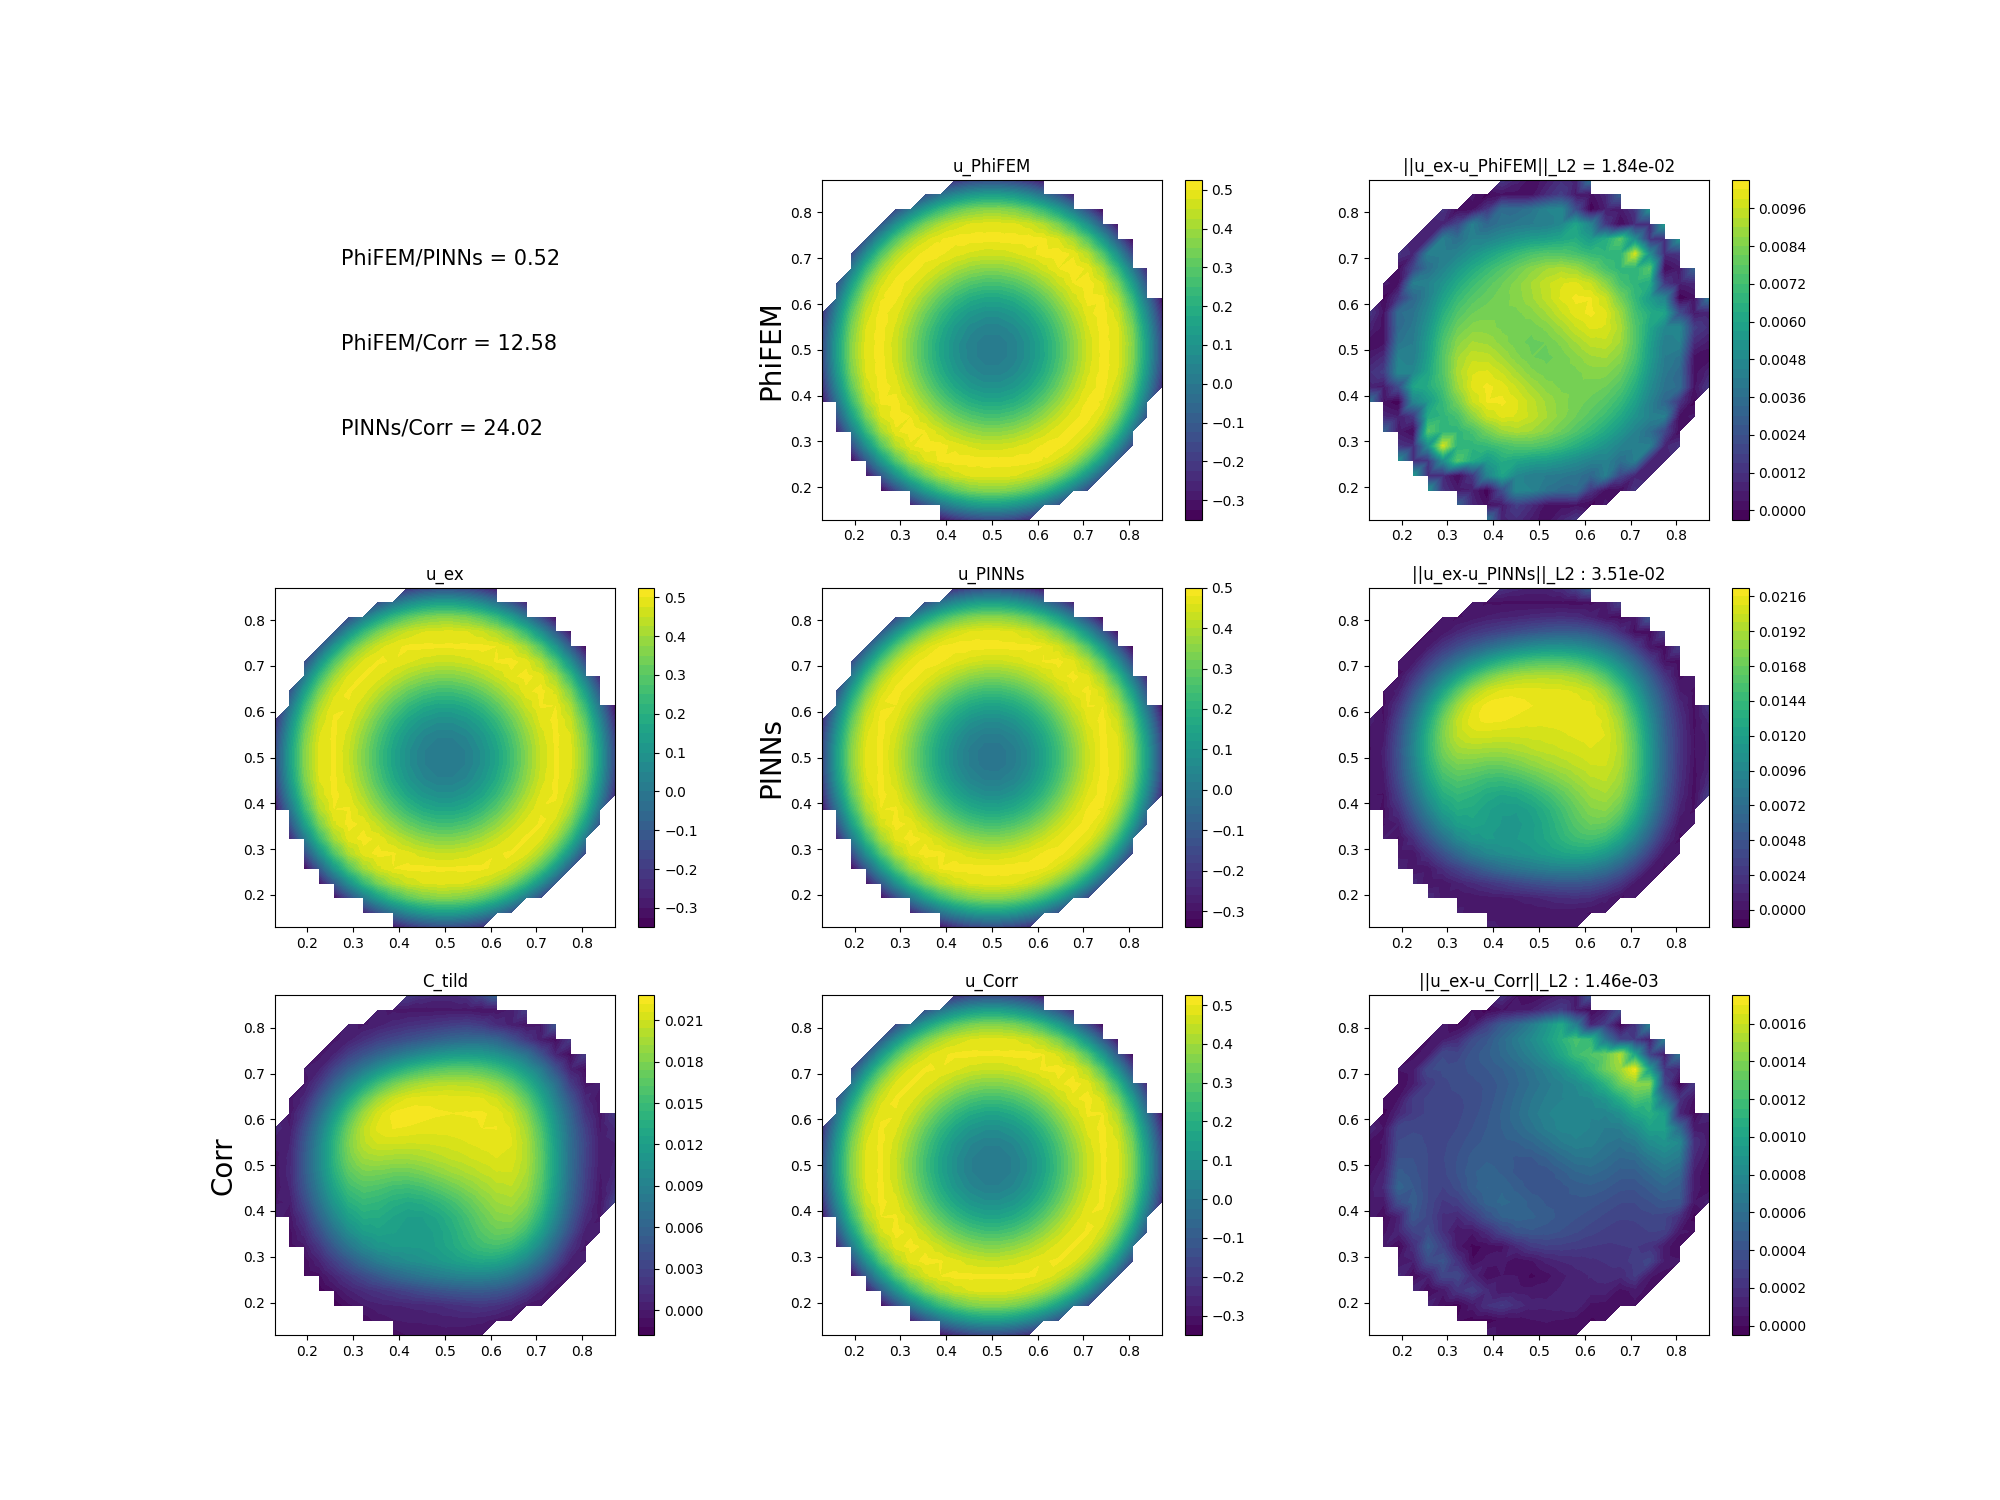
\includegraphics[width=\linewidth]{"corr/corr_phifem_0_exact_bc.png"}
		\caption{Correction avec $\phi$-FEM - Modèle sur $w$.}
		\label{corr_phifem_0_exact_bc}
	\end{figure}
\end{minipage}
\end{document}
	\renewcommand{\insertsectionheadSubtitle}{}
	% \section{New lines of research}

	\section*{Conclusion}

	\begin{frame}{Conclusion}
		\begin{itemize}
			\item The enriched approach provides the same results as the standard FEM method, but with \textbf{coarser meshes}. \\
			$\Rightarrow$ Reduction of the computational cost : DoFs, iterations, execution times.
			\item Theory on linear problems shows that it's the \textbf{derivatives} of the prior that are the most crucial. \; \refappendix{frame:datavspinns} \\
			$\Rightarrow$ PINNs are good candidates for the enriched approach.
			\item The gains obtained on linear problems were much higher. \; \refappendix{frame:linear} \\
			$\Rightarrow$ \textbf{Improved training} of parametric PINN (or Neural Operators).
		\end{itemize}

		\flushright
		\begin{minipage}{0.05\linewidth}
			\flushright
			\rotatebox{90}{\textbf{Preprint (linear)}}
		\end{minipage} \; \begin{minipage}{0.28\linewidth}
		\includegraphics[width=\linewidth]{images/qrcode_paper.pdf}
		\end{minipage}
	\end{frame}

	\BackgroundBiblio
	
	{\setbeamertemplate{footline}{} 	
	\begin{frame}{References}
		\scriptsize
		\bibliography{biblio}

		\flushright
		\begin{minipage}{0.05\linewidth}
			\flushright
			\rotatebox{90}{\textbf{Preprint (linear)}}
		\end{minipage} \; \begin{minipage}{0.28\linewidth}
		\includegraphics[width=\linewidth]{images/qrcode_paper.pdf}
		\end{minipage}
	\end{frame}
	}
	\addtocounter{framenumber}{-1} 
	
	\Background

	% \section{Appendix}
	
	\appendix
	
	% \section{\appendixname~\theappendixframenumber~: Data vs PINNs}\labelappendixframe{frame:fem}

\begin{frame}{\appendixname~\theappendixframenumber~: Data vs PINNs}\labelappendixframe{frame:datavspinns}
	TODO
\end{frame}
\addtocounter{appendixframenumber}{1}

% \section{\appendixname~\theappendixframenumber~: Data vs PINNs}\labelappendixframe{frame:fem}

\begin{frame}{\appendixname~\theappendixframenumber~: Multiplicative approach}\labelappendixframe{frame:mult}
	TODO
\end{frame}
\addtocounter{appendixframenumber}{1}


\begin{frame}{\appendixname~\theappendixframenumber~: Non-linear problems}\labelappendixframe{frame:nonlinear}
	TODO
\end{frame}
\addtocounter{appendixframenumber}{1}
	
\end{document}
